% This is based on the LLNCS.DEM the demonstration file of % the LaTeX macro
% package from Springer-Verlag % for Lecture Notes in Computer Science, version
% 2.4 for LaTeX2e as of 16. April 2010
%
% See http://www.springer.com/computer/lncs/lncs+authors?SGWID=0-40209-0-0-0
% for the full guidelines.
\documentclass{llncs}
\usepackage{graphicx}
\graphicspath{ {./assets/}, {./assets/protocol/}, {./assets/tx-graph/} }

\usepackage{enumitem}
\setlist[enumerate]{itemsep=2mm}

\usepackage{dirtytalk}
\usepackage{minted}
\usepackage{amsmath}
\usepackage{pdflscape}
\usepackage[pass]{geometry}

%
% Tables
% --------
\usepackage[table]{xcolor}
\usepackage{hhline}
\usepackage{booktabs} % much better tables
\usepackage{multirow} % allows to fuse rows
\usepackage{array}    % manipulate array
\usepackage{tabularx} % better tables

% Define new tabularx column types:
%  - R: streteched right aligned
%  - C: stretched centered
%  - N: left aligned, specified space
\newcolumntype{R}{>{\raggedleft\arraybackslash}X}
\newcolumntype{C}{>{\centering\arraybackslash}X}
\newcolumntype{N}[1]{>{\raggedleft\arraybackslash}p{#1}}
\newcolumntype{S}{>{\hsize=.5\hsize}C}

% Set row height multiplicator to provide more breathing space
\renewcommand{\arraystretch}{1.5}

\usepackage[backend=biber]{biblatex}
\addbibresource{bibliography.bib}

\pagestyle{plain}
\setcounter{page}{1}
\pagenumbering{arabic}

\begin{document}

\title{Partially Non-Interactive and Instantaneous Bitcoin One-way Payment
Channel}

\author{Thomas Shababi\inst{1} \and Jo\"el Gugger\inst{1} \and Daniel Lebrecht\inst{1}}

\authorrunning{Thomas~S.~Shababi et al.}
\tocauthor{Thomas~S.~Shababi, Joel Gugger, and Daniel Lebrecht}

\subtitle{{\normalsize\today}}

\institute{TrueLevel SA, Neuch\^atel, Switzerland\\ \email{\{tom, joel, d\}@truelevel.io}}

\maketitle

\begin{abstract} The most significant challenge for Bitcoin in the coming years
  is scalability. Currently, Bitcoin enforces a 1 Megabyte block-size limit. On
  average every 10 minutes a new block is discovered. That produces a payment
  network limited to $\approx7$ transactions per second, and with delayed (and
  unknown) transaction confirmation times. This is not sufficient in comparison
  to the currently deployed payment infrastructure such as credit card
  processors, which allows tens of thousands of transactions per second. To
  address this, there are some proposals to modify (i) the transaction structure
  (such as in SegWit), (ii) the block-size limit (such as SegWit2x) or even
  (iii) build a second layer on top of the Bitcoin protocol (such as the
  Lightning Network). Following the rational of second layer solutions, we
  propose a retail-ready, one-way payment channel that enables two parties to
  transact mostly off-chain, thus reducing the number of on-chain transactions
  and operational cost, while remaining secure and trustless. After the channel
  is opened for a few blocks, payment channel transactions are instantaneous and
  irreversible, and do not rely on the seemly random block arrival times. At all
  times, only one of the parties (the money receiver) must stay online to secure
  the channel integrity. The money receiver can redeem his channel funds on
  chain with no delay at all times. The money sender does not have to perform
  any action to secure its funds. \keywords{Crypto-currencies, Bitcoin, Payment
    channels, State channels, Threshold ECDSA signatures}
\end{abstract}
%
\section{Introduction} Decentralized crypto-currencies such as Bitcoin
\cite{Nakamoto_bitcoin} and its derivatives employ a special decentralized
public append-only log based on proof-of-work called the \textit{blockchain}. In
a decentralized crypto-currency, users transfer their funds by publishing
digitally signed transactions. Transactions are confirmed only when they are
included in a block that extends the longest chain, which is validated and
accepted by other nodes of the network. To get the right to include a block to
the blockchain, bitcoin miners solve a proof-of-work problem that can only be
solved by brute force computation. For its work, the miner has the right to
create some bitcoins. And this is the only source of bitcoins in the
network, thus all bitcoins can be tracked down to its creation by miners.

The blockchain protects against state transitions that are conflicting with each
other, for example \textit{double-spending} attempts. Since the money is
digital, nothing prevents a user to send the same digital funds to two different
recipients at the same time. Although a malicious bitcoin owner potentially can
sign over the same funds to multiple receivers through multiple transactions,
eventually only one transaction will be approved and added to the publicly
verifiable blockchain. The whole history all coins, from creation by miners to
the present state must be unambiguous, and verifiable by all nodes.

The bitcoin blockchain is slow, growing on average at 1 MB per 10 min velocity.
Most of its security model depends on transactions getting included to the
blockchain within a certain amount of time. Thus a block space market developed
to ensure that transactions get confirmed on chain. Users pay a variable miners
fee to get their transactions prioritized by the miners. In December 2017, a
large fraction of users payed over USD \$30 in fees to get their transactions
quickly confirmed.

Scalability is one of the most significant challenges in blockchain systems. As
mentioned before, some proposals are focused on the blockchain data
\cite{SegWit, SegWitBIP, SegWit2x} structures and the consensus layer, others
\cite{lightningNetwork} are focused on a second layer of transactions where
transactions are created off-chain and the blockchain itself is used as a
conflict resolution system and source of truth. These proposals are called
payment channels, or layer-two applications, and provide a wide range of
advantages. The idea of payment channels was suggested by Satoshi in an email
to Mike Hearn. Since then, various propositions to construct such structures
have been proposed.

\subsection{The value of unidirectional channels}
Streaming payments in a retail context are mostly unidirectional. As an example,
most people receive their salaries once a month---a large incoming payment---and
across the rest of the month they send small outgoing payments to cover their
living costs.

Thus on average the number of incoming transactions, $N(tx_{in})$, is far
lesser than the number of outgoing transactions, $N(tx_{out})$

$$N(tx_{in}) \ll N(tx_{out})$$

In bitcoin, the transaction cost is related to the size of the transaction in
bytes and not the amount transacted in bitcoin. Thus small or large payments
incurs approximately the same transaction cost.

When decreasing the number of on-chain payments, the most weighted variable thus
is $N(tx_{out})$, and it should be minimized. Interestingly, unidirectional
payment channels do minimize $N(tx_{out})$, although they have no effect on
$N(tx_{in})$, in the case.

However, the previous statement assumes that all payments go to the same
recipient. Thus here the client, hereinafter Carol (the money sender), wants to
buy goods or services from a business, Bob (the money receiver). For a channel
to generate savings, Carol and Bob should have a lasting relationship. For
example, Bob sells goods or services to Carol repeatedly within a small time
interval.

\subsection{The issues of bidirectional channels} Bidirectional payment channels
impose the burden upon both parties to police the channel by listening to
the network at all times and submitting transactions to enforce the correct
state gets on-chain \cite{lightningNetwork}, which greatly increases the
complexity for the both participants. This property make such channels
less practical for real world retail use cases.

\subsection{Wish-list for a channel to be used in retail settings } On this
work, we will focus on a partially non-interactive (for the client), partially
instantaneous (for the business), one-way channel that is more suitable for the
retail context (loosely based on \cite{YoursLightningProtocol,
lightningNetwork}).

It is of general believe that bitcoin cannot be used for retail. Transaction
cost is too high and confirmation times are too long. As it is popularly stated
``You cannot pay for your coffee with bitcoin!'' And in 10 years time, why
should anyone have to validate your coffee payment?

With that in mind, we acknowledge the following constraints to be essential for
a channel to become practical for usage in retail settings.

\begin{enumerate}[label=(\roman*)]
\item Channel transactions finality must be reached instantaneously---It must
  not require waiting for a block to be mined. That is, Bob knows for sure that
  he received a payment, and that it is irreversible, and should feel confident
  to handle the products to Carol and let her walk off his store.
\item Few on-chain transactions---Cheap to make large numbers of small payments
  with only a couple of on-chain transactions. Additionally, on-channel
  transactions are private. Thus the 10-year old coffee purchase will be hidden
  together with other purchases on a single bitcoin transaction.
\item No counter-party risk---Any party can disappear from existence and the
  other party's funds stay safe, and are redeemable at any time. Each party must
  be able to single-handedly get their unspent or received funds by publishing
  on chain transactions at all times without the need of the other party to
  cooperate.
\item Bob must be able to settle at any time, and immediately be able to spend
  the funds---the funds owed to Bob are fully liquid at all times---The goods
  and services were provided to Carol, but Bob's money is locked up in the
  channel and he should be able to redeem his funds with no delay whenever he
  needs it to provide liquidity to his business.
\item Bob must not lock funds upfront for each of the clients---It is unfeasible
  and costly for retail businesses to have to stake funds for each of their
  several clients.
\item Carol does not have to watch over her deposited funds---She deposits the
  money and forgets about it. It is safe in there at all times.
\end{enumerate}

The currently available proposals of bidirectional channel do not fulfill the
last 3 constraints of the list, and therefore are unsuitable for the task. On
this work, we specifically designed a payment channel construct that fulfills
the entire list of the above constraints. To achieve that we focused on a
unidirectional payment channel. Further characteristics of the channel are
listed below.

\begin{enumerate}[label=(\roman*)]
\item The channel should stay open for an unlimited amount of time, like a
checking bank account, and Carol has the option to close the account at any time
and take its funds back.
\item Carol, who has locked funds in a channel with Bob, must be able to
withdraw an arbitrary amount out of her channel balance without closing it, with
the Bob's cooperation. In case Bob does not cooperate, then she has to close the
channel.
\item Bob is expected to stay online to stay safe. He runs a business afterall
and can be expected to incur the cost to secure his funds.
\item If Bob needs to send money to some clients, it is assumed that these
transactions are regular on-chain transactions or via other channels.
\end{enumerate}

\subsection{Incentive structure} From a game theoretical perspective, Carol (or
Bob) should always submit the transaction that pays herself (or himself) the
most. On a one-way channel whereby Carol locked funds initially, the transaction
that pays Carol the most is the first refund transaction---all the money goes
back to her. While for Bob, the one that pays him the most will always be the
last one---interestingly, by design the last state is always the valid one. This
asymmetry promotes Bob to behave correctly and submit the last state even in the
absence of policing by Carol. Thus the only party of the channel that must be
policed is Carol, as she will always have the incentive to publish old state
that pays her more. This feature is used to produce a practical channel in which
clients do not have to stay online.

\subsection{Transaction malleability} The scheme we present requires a proper
fix to transaction malleability such as SegWit \cite{SegWit, SegWitBIP}.
It is assumed that a chain of unconfirmed transactions can be creates and
trusted without breaking the security model defined above.

\section{Building Blocks} In the following, the concepts and sub-protocols used
in this work are described in more detail.

\subsection{Channel State} The channel state is expressed by two indexes $i$ and
$n$, hereinafter also $\texttt{Channel}_{i,n}$. Both indexes are independent and
can only be positively incremented, one at a time, with increments of +1 on i
only or on n only. Each increment represents a state transition (or a move) in
the channel state. Index $i$ represents the offset of the multisig address where
the channel's funds are locked. Index $n$ represents the offset used to create
the revocation secrets, which are later used in smart contracts to revoke the
past off-chain transactions.

A channel state always depends on an account $a$, this account is defined when
the channel is created between the client and the server and never changes
during its life. We need to share public hierarchical deterministic addresses
between the client and the server. Let's define the hierarchical deterministic
Bitcoin account path as:
\begin{eqnarray*} \forall a \geq 2,& \exists \texttt{xPriv}_{a} &\mid
\texttt{xPriv}_{a} = \texttt{m/44'/0'/a'}\\ \forall a \geq 2,& \exists
\texttt{xPub}_{a} &\mid \texttt{xPub}_{a} = \texttt{m/44'/0'/a'}
\end{eqnarray*}

For a given account $a$ at $\texttt{Channel}_{i,n}$, the protocol and
transactions depend on the private multi-signature node $\Pi$, the public
multi-signature node $\pi$, the private revocation node $\Omega$, the public
revocation node $\omega$, and the private secret node $\Theta$. Let's define
these nodes as:
\begin{eqnarray*} \Pi_{i} &= \texttt{xPriv}_{a} &\texttt{/0/i}\\ \pi_{i} &=
\texttt{xPub}_{a} &\texttt{/0/i}\\ \Omega_{i} &= \texttt{xPriv}_{a}
&\texttt{/1/i}\\ \omega_{i} &= \texttt{xPub}_{a} &\texttt{/1/i}\\ \Theta_{n} &=
\texttt{xPriv}_{a} &\texttt{/2'/n'}
\end{eqnarray*}

Unlike $\Theta_{n}$, the nodes $\Pi_{i}$, $\pi_{i}$, $\Omega_{i}$ and
$\omega_{i}$ are not hardened derivations. It cannot be done because the public
keys $\pi_{i}$ and $\omega_{i}$ must be computed from $\texttt{xPub}_{a}$.

\subsubsection{Channel Dimensions} The channel dimension, noted
$|\texttt{Channel}|$, depends of the number of indexes present in the state.
Let's define the channel dimension:
\[ N = |\texttt{Channel}_{i,n}| = 2
\]

\subsubsection{Revocation Secret} The revocation sercret, noted $\Phi_{i,n}$,
corresponds to the state $\texttt{Channel}_{i,n}$ and depends on the secret
$\Theta_{n}$ and the revocation key $\Omega_{i}$.
\[ \Phi_{i,n} = \texttt{HMAC}(\Theta_{n}, \Omega_{i})
\]

The secret is the \texttt{HMAC} of $\Theta_{n}$ and $\Omega_{i}$. Both indexes
are used to protect Carol from the Old Settlement Attack With Weak Secret (see
\ref{sssec:oldSettlementAttack}).

\subsection{Smart Contracts}
\label{ssec:SmartContracts} Two types of smart contracts are used in the payment
channel scheme. The first one is a standard 2-out-of-2 multi-signature script
and the second is a custom script used to prevent the client from broadcasting
old transactions.

\subsubsection{Multisig Contract} The multi-signature contract at
$\texttt{Channel}_{i,n}$, hereinafter $\texttt{Multisig}_{i}$, can be
constructed with Carol's $\pi_{i}$ key, and Bob's $\pi_{i}$ key. Let's define
the $\texttt{Multisig}_{i}$ script:

\begin{minted}[escapeinside=||,mathescape=true]{text}
OP_2 <|$\pi_{i}^{carol}$|> <|$\pi_{i}^{bob}$|> OP_2 OP_CHECKMULTISIG
\end{minted}

\subsubsection{Revocable PubKey Contract} Bob and Carol may wish to make an
output to Carol which Carol can spend after a timelock and Bob can revoke if it
is an old state. The next contract, for $\texttt{Channel}_{i,n}$, uses Carol's
$\omega_{i}$ key, Bob's $\omega_{i}$ key, and Carol's secret $\Phi_{i,n}$.

%TODO add ref to checksiquenceverify

\begin{minted}[escapeinside=||,mathescape=true]{text}
OP_IF
  <|$\omega_{i}^{carol}$|> OP_CHECKSIG
  <timelock> OP_CHECKSEQUENCEVERIFY OP_DROP
OP_ELSE
  <|$\omega_{i}^{bob}$|> OP_CHECKSIGVERIFY
  OP_HASH160 <Hash160(|$\Phi_{i,n}$|)> OP_EQUAL
OP_ENDIF
\end{minted}

With this contract Carol can spend this output after the timelock with the
script signature:

\begin{minted}[escapeinside=||,mathescape=true]{text}
<|$\Omega_{i}^{carol}$| signature> OP_TRUE
\end{minted}

In case Carol broadcasts an older transaction, Bob can revoke it with the script
signature:

\begin{minted}[escapeinside=||,mathescape=true]{text}
<Carol's |$\Phi_{i,n}$|> <|$\Omega_{i}^{bob}$| signature> OP_FALSE
\end{minted}

Bob has a head start during which, if he knows the secret $\Phi_{i,n}$ generated
by Carol, he can spend the money while Carol cannot. This mechanism prevents
Carol from broadcasting older transactions which do not match the current
$\texttt{Channel}_{i,n}$ state.

\subsection{Transactions} A transaction is represented as
$\texttt{Transaction}_{<>}^{i,n}$, where $\texttt{Transaction}$ denotes the name
of the transaction, the superscript indexes represent the transaction's state
dependencies---on this example $i$ and $n$---and the subscript represents who
has already signed the transaction---denoted by the $<>$ for no signatures. If a
transaction is signed by Carol the transaction is noted
$\texttt{Transaction}_{<carol>}^{i,n}$. Transactions that appear in blue on the
figures are fully signed and only available to Carol and in red are fully signed
and only available to Bob, thus only the specific parties can broadcast the
transaction.

\subsubsection{Funding Transaction} The funding transaction, hereinafter
$\texttt{FundingTx}_{<>}^{i}$, is the transaction sending funds to the first
multisig address. This transaction depends only on the state index $i$ used by
the multisig contract and is fully signed as soon as Carol signs it.

A funding transaction is never broadcast by Carol until she possesses the
corresponding refund transaction that allows her to get her money back off the
channel. This refund transaction has only one output that goes to the revocation
contract. To be able to revoke this contract, Bob has to know the secret
$\Phi_{i,n}$. So if no channel transactions have ever been made, Bob cannot
revoke the contract.

\begin{figure}[t]
  \centering 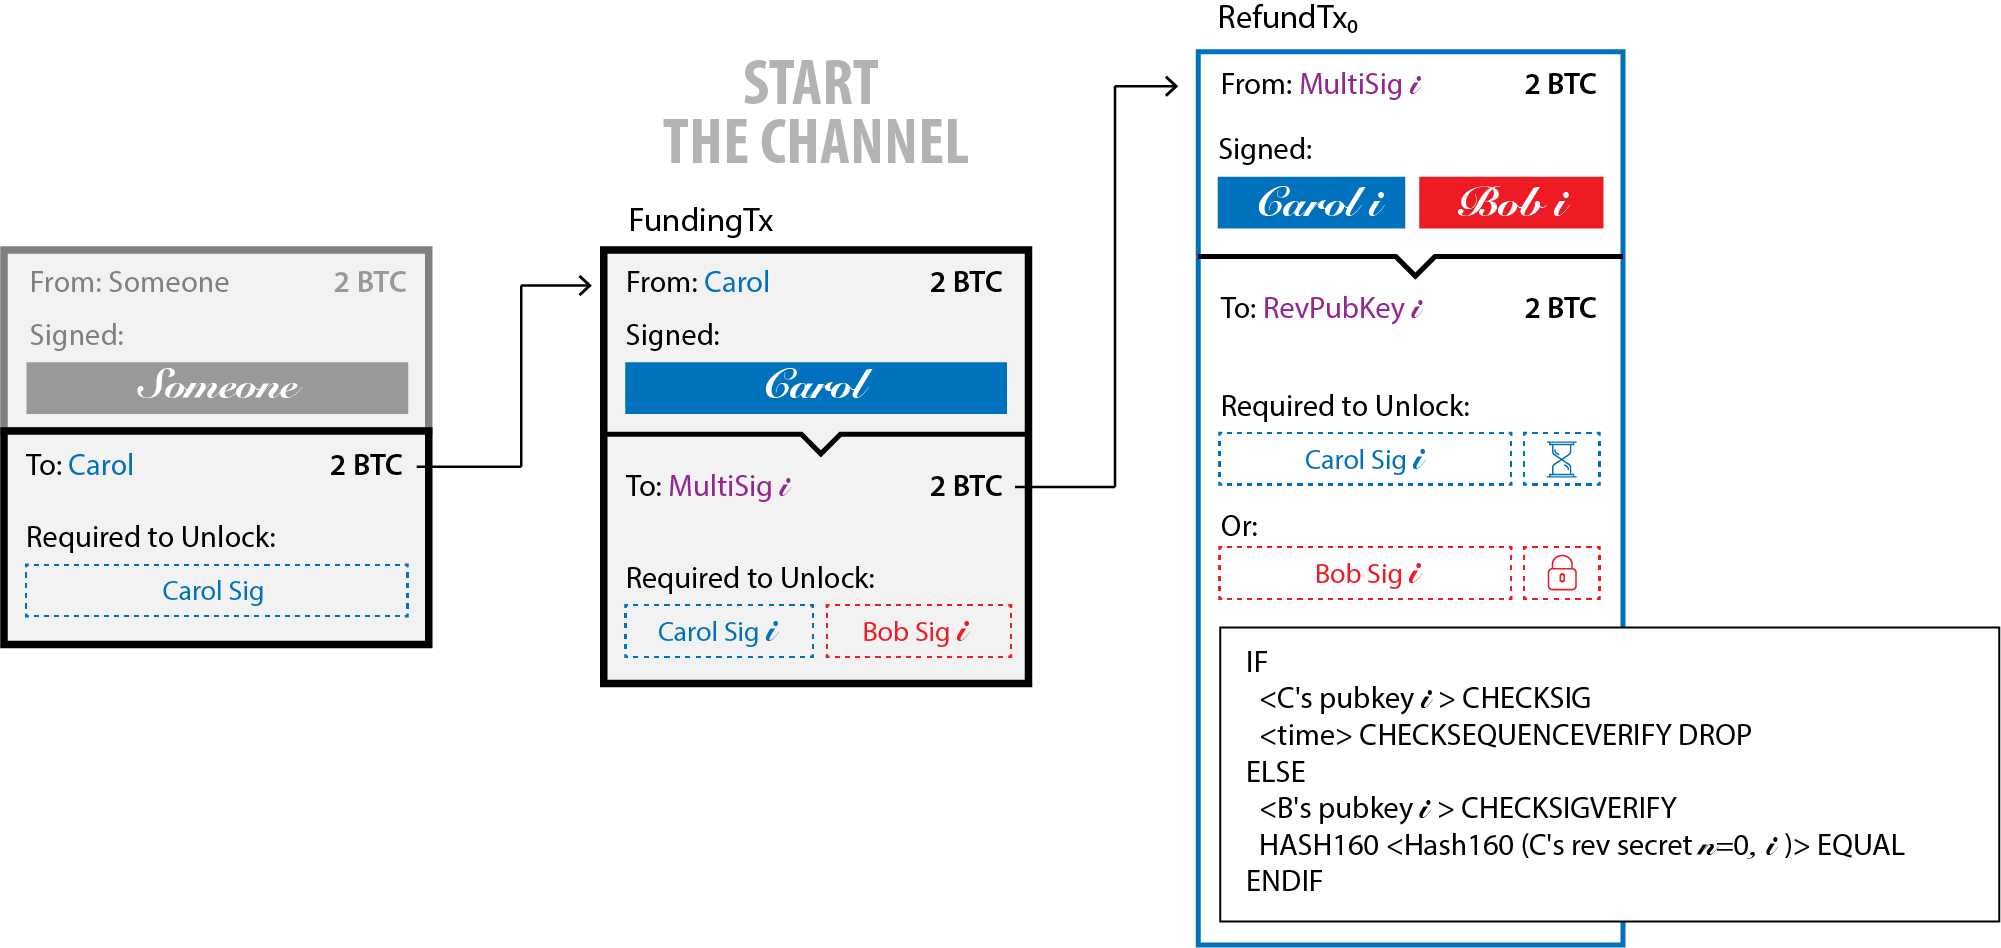
\includegraphics[width=1\textwidth]{FundingRefundTx}
  \caption{Funding transaction that starts the channel by sending money in the
first multisig address. Along with the first refund transaction that allows
Carol to close the channel if no transactions are made.}
\end{figure}

\subsubsection{Refund Transaction} The refund transaction, hereinafter
$\texttt{RefundTx}_{<>}^{i,n}$, is a transaction that keeps track of the
balances of Carol and Bob at $\texttt{Channel}_{i,n}$. It also allows Carol to
close the channel if Bob does not respond or does not cooperate anymore. This
transaction has one or more inputs and two outputs. The number of inputs depends
on how many unspent transaction outputs are available at the
$\texttt{Multisig}_i$ address. The first output represents the amount still
owned by Carol, and the second, if present, is the amount owned by Bob. Bob
might have a channel balance equal to zero, in which case the second output is
excluded, such as when starting the channel, or right after Bob settles the
channel.

Carol's balance is sent to a revocation contract corresponding to the channel
state. This prevents Carol from broadcasting an old refund transaction such as
$\texttt{RefundTx}_{<>}^{i,n-1}$. The amount owned by Bob is sent directly to
Bob's address. The refund transaction is broadcast by Carol so the fees are
substracted from the first output, owned by Carol.

\begin{figure}[t] \centering 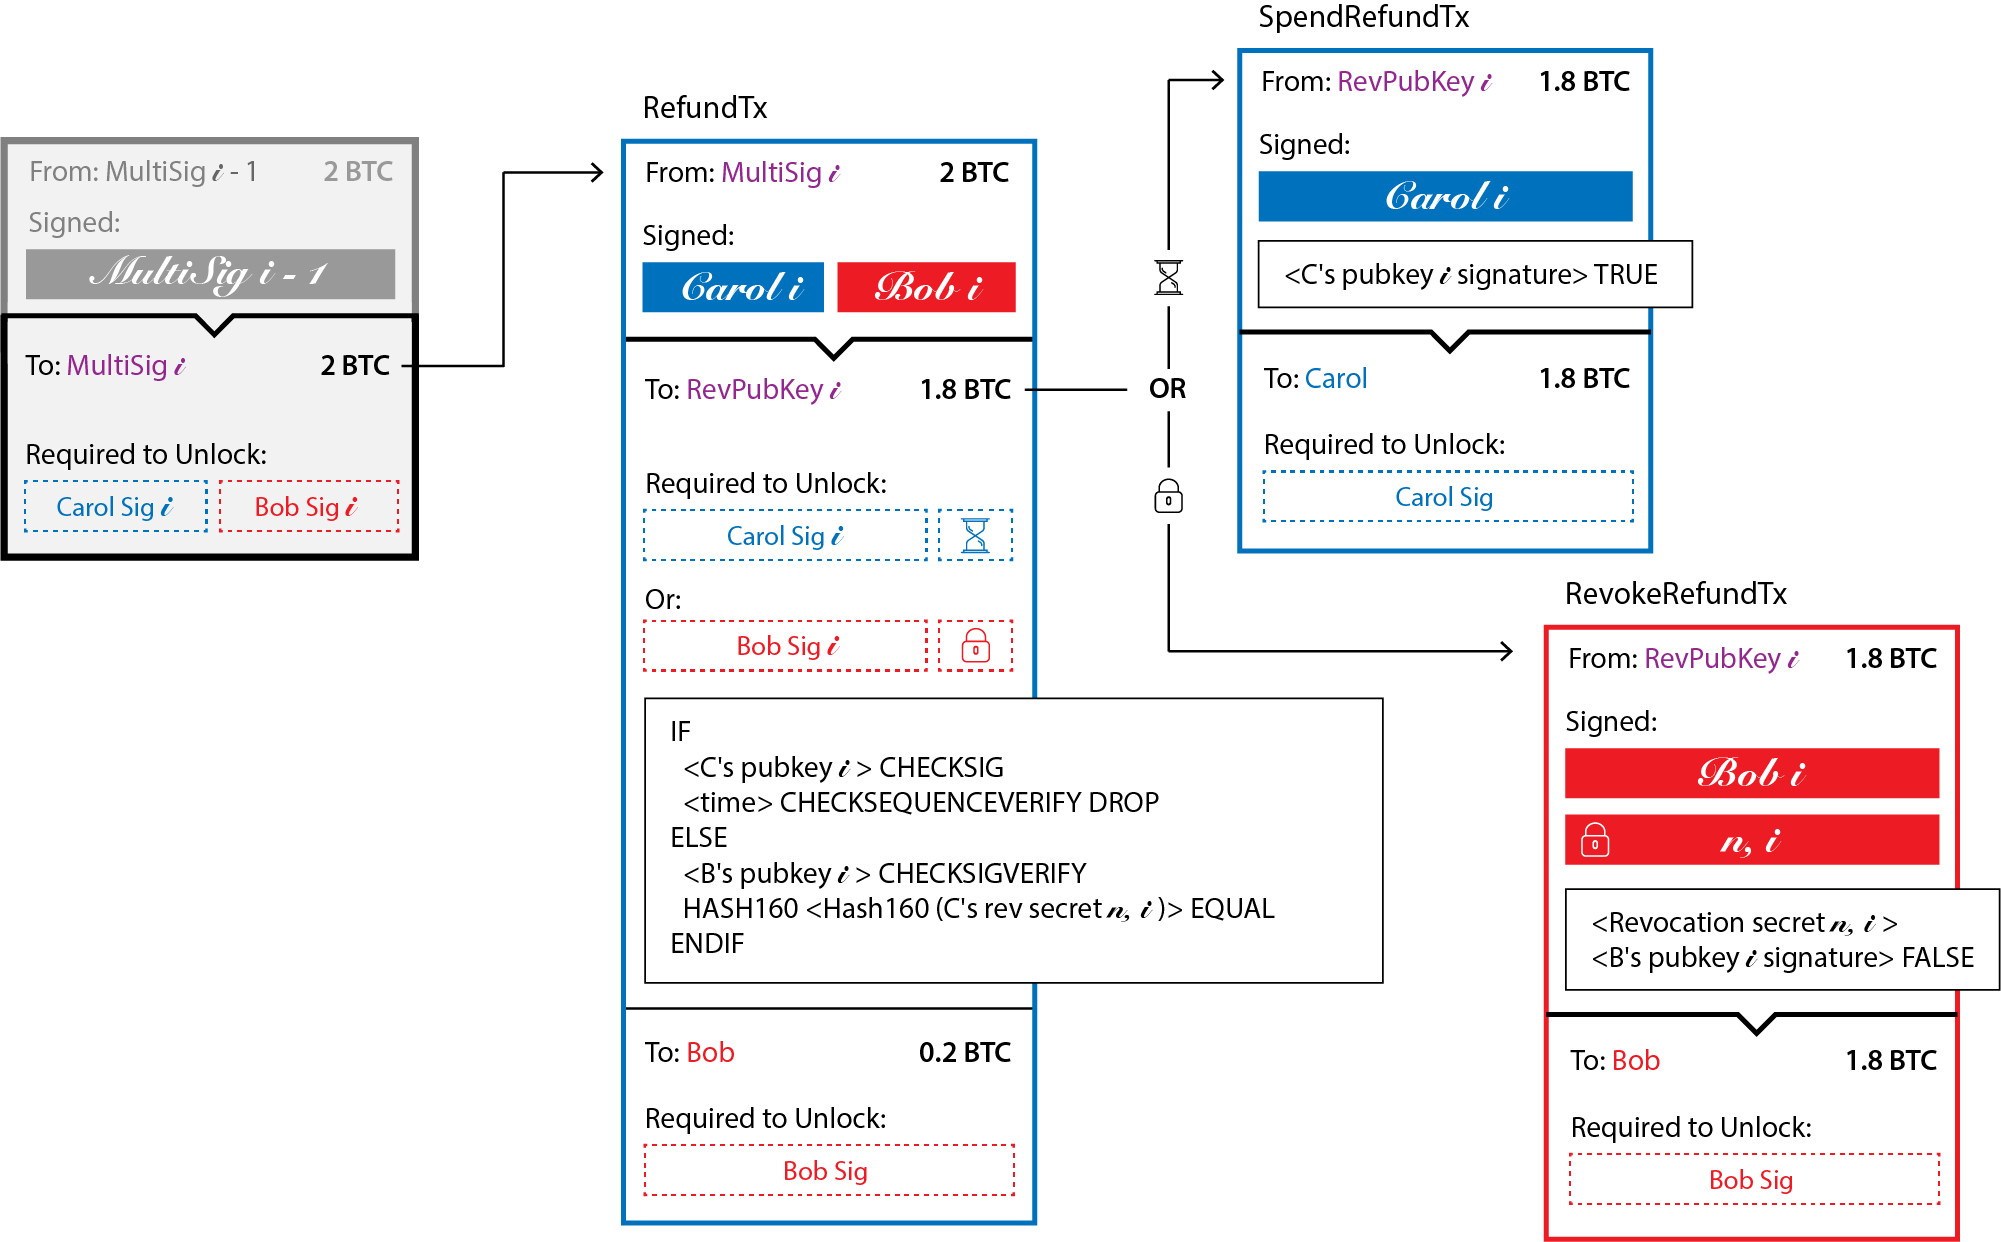
\includegraphics[width=1\textwidth]{RefundTx}
  \caption{Refund transaction based on the current multisig address with the
associated spend and revoke transactions. The former allows Carol to get her
money back and the latter Bob to revoke the contract if he knows the secret.}
\end{figure}

Because a refund transaction spends funds from a multisig address, it must be
signed by both Carol and Bob to be considered valid. The revocation contract
used in the Carol's output can be spent with a \textit{spend-refund} transaction
after a \textit{timelock} delay. She only needs to sign the output with her
$\Omega_{i}$ key to unlock the funds. Bob can directly revoke the contract,
without delay, if he knows the secret $\Phi_{i,n}$ and signs with his
$\Omega_{i}$ key.


\subsubsection{Settlement Transaction} The settlement transaction, hereinafter
also mentioned as $\texttt{SettlementTx}_{<>}^{i,n}$, is a transaction that
keeps track of Carol and Bob's balances at $\texttt{Channel}_{i,n}$ and allows
Bob to settle the channel without closing it. Because the settlement transaction
spends the funds from the multisig address, both Carol and Bob need to sign to
consider the transaction as valid. Fees are substracted from Bob's output,
because he is responsible for broadcasting the transaction and settling the
channel.

A settlement transaction always has one output that sends Bob's balance directly
to his address and one output that sends the remaining funds to the next
multisig address $\texttt{Channel}_{i+1,n}$. Because the funds are sent to the
next multisig address, a post settlement refund transaction is created; Carol
needs a way to get her money back off the channel. This transaction has the same
structure as the first refund transaction---one output to the next revocation
contract---because the funds owned by Bob, in this case, are already settled.

If Bob broadcasts the fully signed settlement transaction, Carol has two
options:
\begin{enumerate}[label=(\roman*)]
\item continue to transact on the channel with the new multisig address; or
\item close the channel with her post settlement refund transaction.
\end{enumerate} It is worth noting that the secret for the revocation contract
is $\Phi_{i+1,n}$, so in the case of a new channel transaction
$\texttt{Channel}_{i+1,n}$ becomes $\texttt{Channel}_{i+1,n+1}$, and then the
secret for $\texttt{Channel}_{i,n-1}$ is shared:
\[ \Phi_{i,n-1}(\texttt{Channel}_{i+1,n+1}) = \Phi_{i+1,n}
\]

\subsubsection{Post Settlement Refund Transaction} The post settlement refund
transaction aims to spend funds from the next multisig address directly to a
revocation contract. As explained before, this contract is not revocable by Bob
if no transactions are made after the settlement transaction. However, when
Carol sends an amount to Bob, she shares the secret needed to revoke the
contract. Therefore she cannot broadcast this transaction that is now attached
to an old state.

\begin{figure}[t] \centering 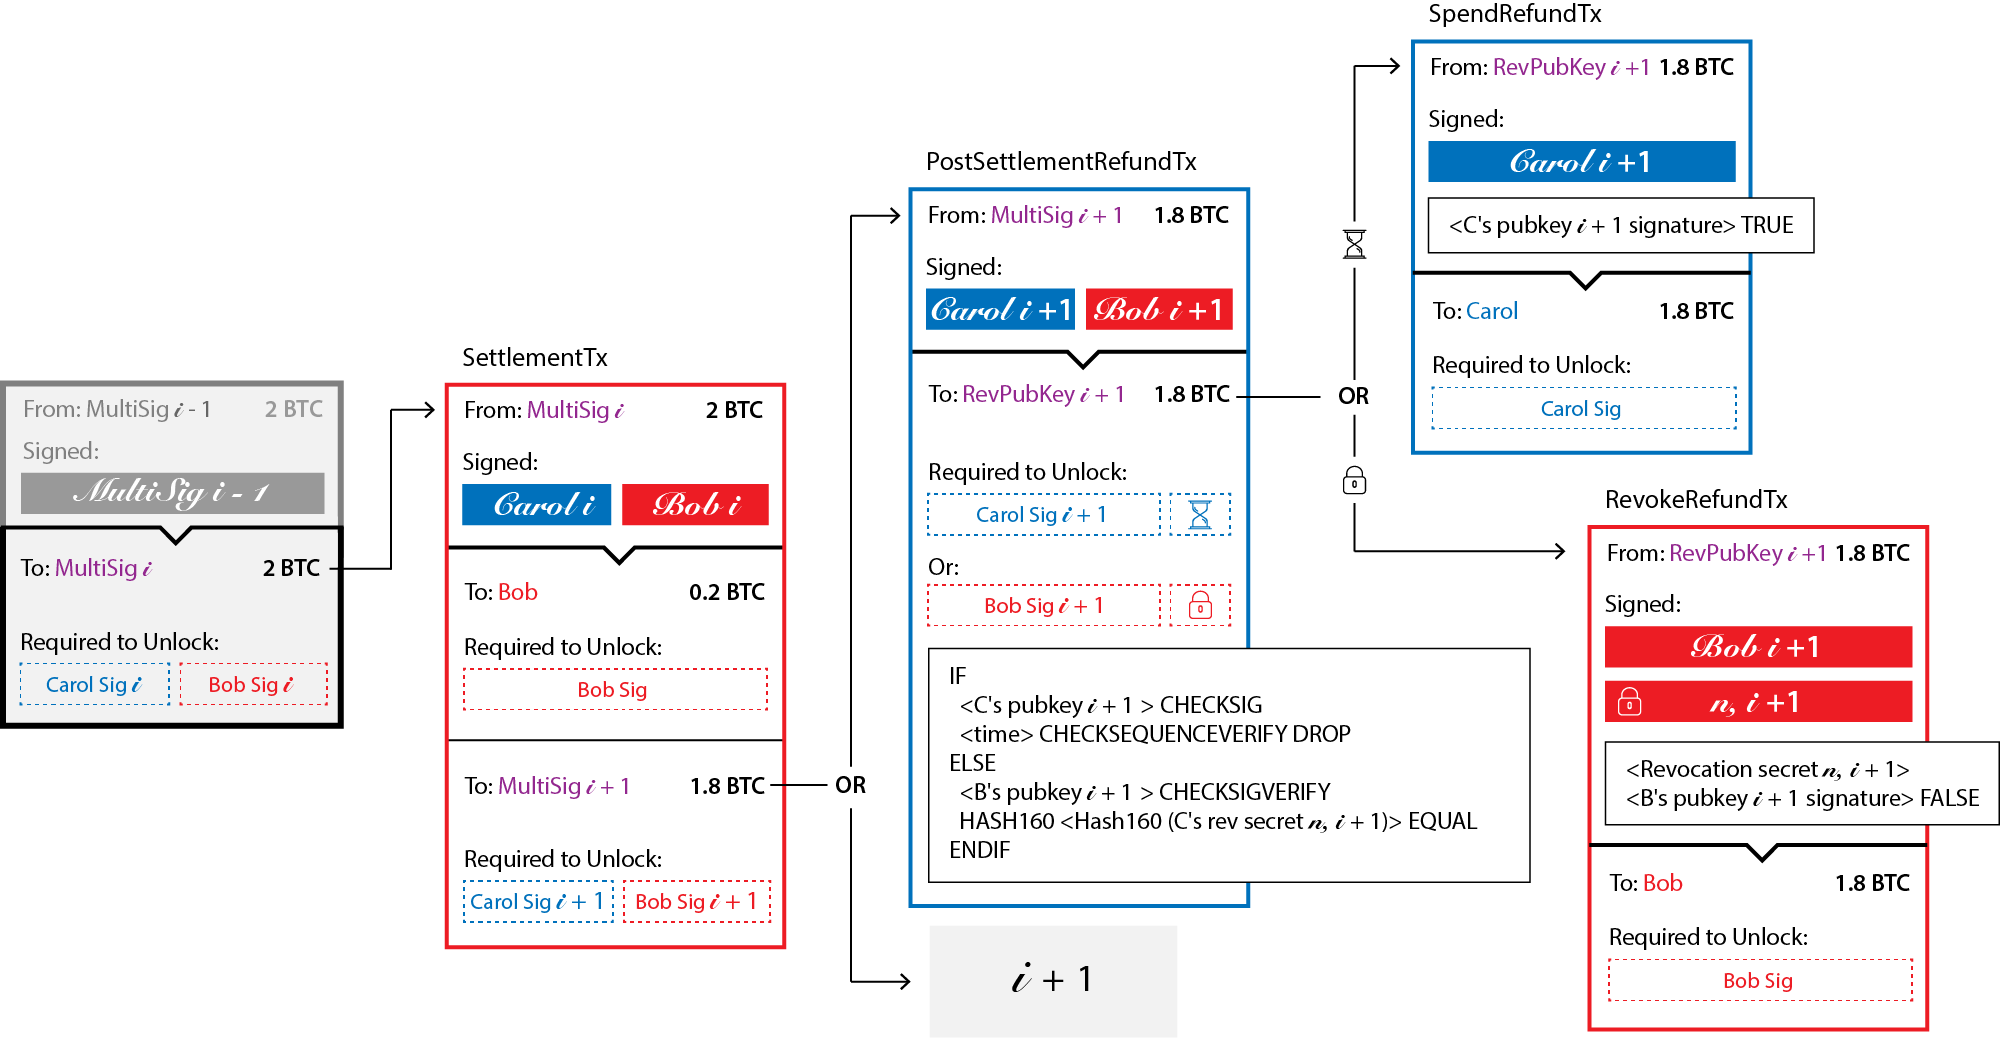
\includegraphics[width=1\textwidth]{SettlementTx}
  \caption{Settlement transaction that allows Bob to settle the channel, moving
the remaining funds to the next multisig address with the post settlement refund
transaction. The latter transaction allows Carol to close the channel directly
after the settlement.}
\end{figure}

\subsubsection{Withdraw Transaction} The withdraw transaction, hereinafter
$\texttt{WithdrawTx}_{i}$, is a transaction that allows Carol to take an
arbitrary amount of money out of the channel. This amount is sent to an
arbitrary address specified by Carol. For this, she has to ask Bob for his
cooperation. This transaction is not auto-generated when Carol sends money to
Bob, both have to be online to create this transaction.

\begin{figure}[t] \centering 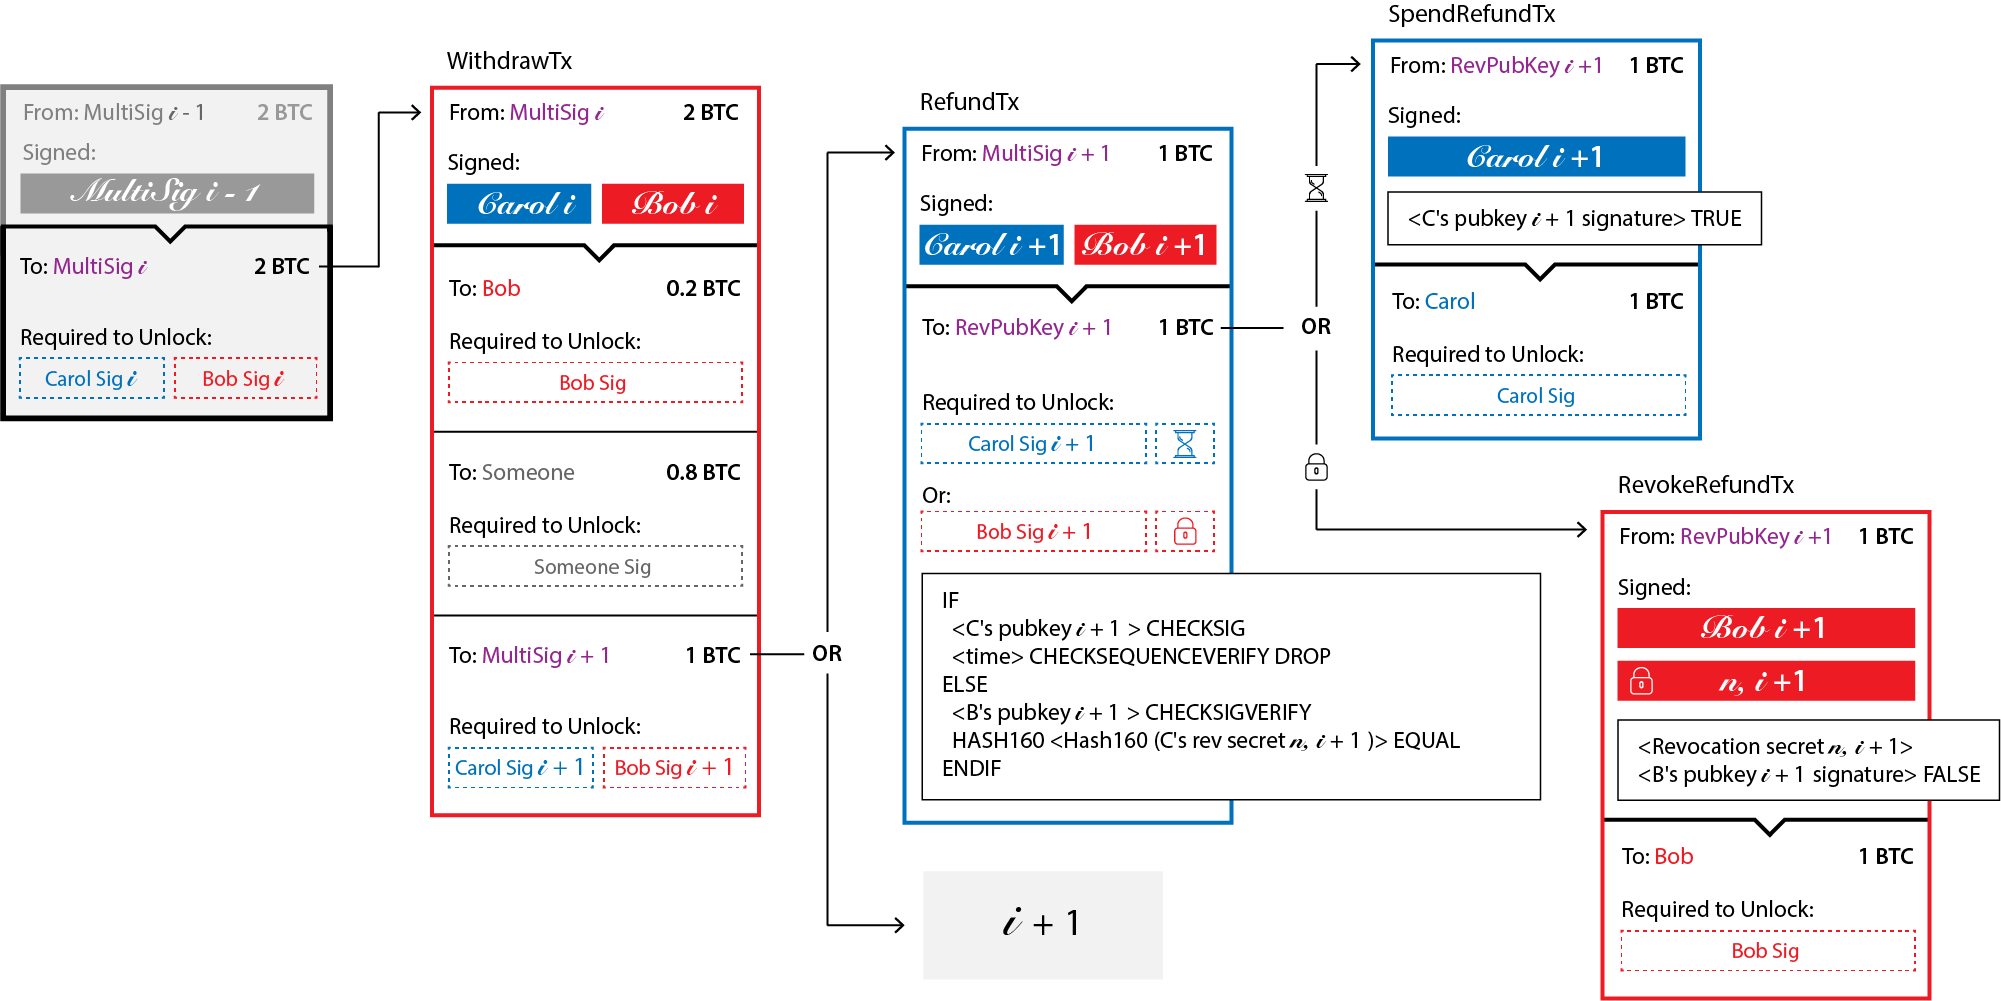
\includegraphics[width=1\textwidth]{WithdrawTx}
  \caption{Withdraw transaction that allows Carol to take money out the channel,
pay Bob, and move the remaining funds into the next multisig address. A refund
transaction is created to allow Carol to recover her funds after the withdraw if
no transaction is made. The refund transaction can be spent by Carol with a
spend refund transaction and cannot be contested with the revoke refund
transaction if no other transaction is made. If the state moves to
$\texttt{Channel}_{i+1,n+1}$, again, the secret for $\texttt{Channel}_{i,n-1}$
is shared, then Bob knows $\Phi_{i,n-1}(\texttt{Channel}_{i+1,n+1}) =
\Phi_{i+1,n}$ and can revoke.}
\end{figure}

\begin{figure}[H]
  \centering 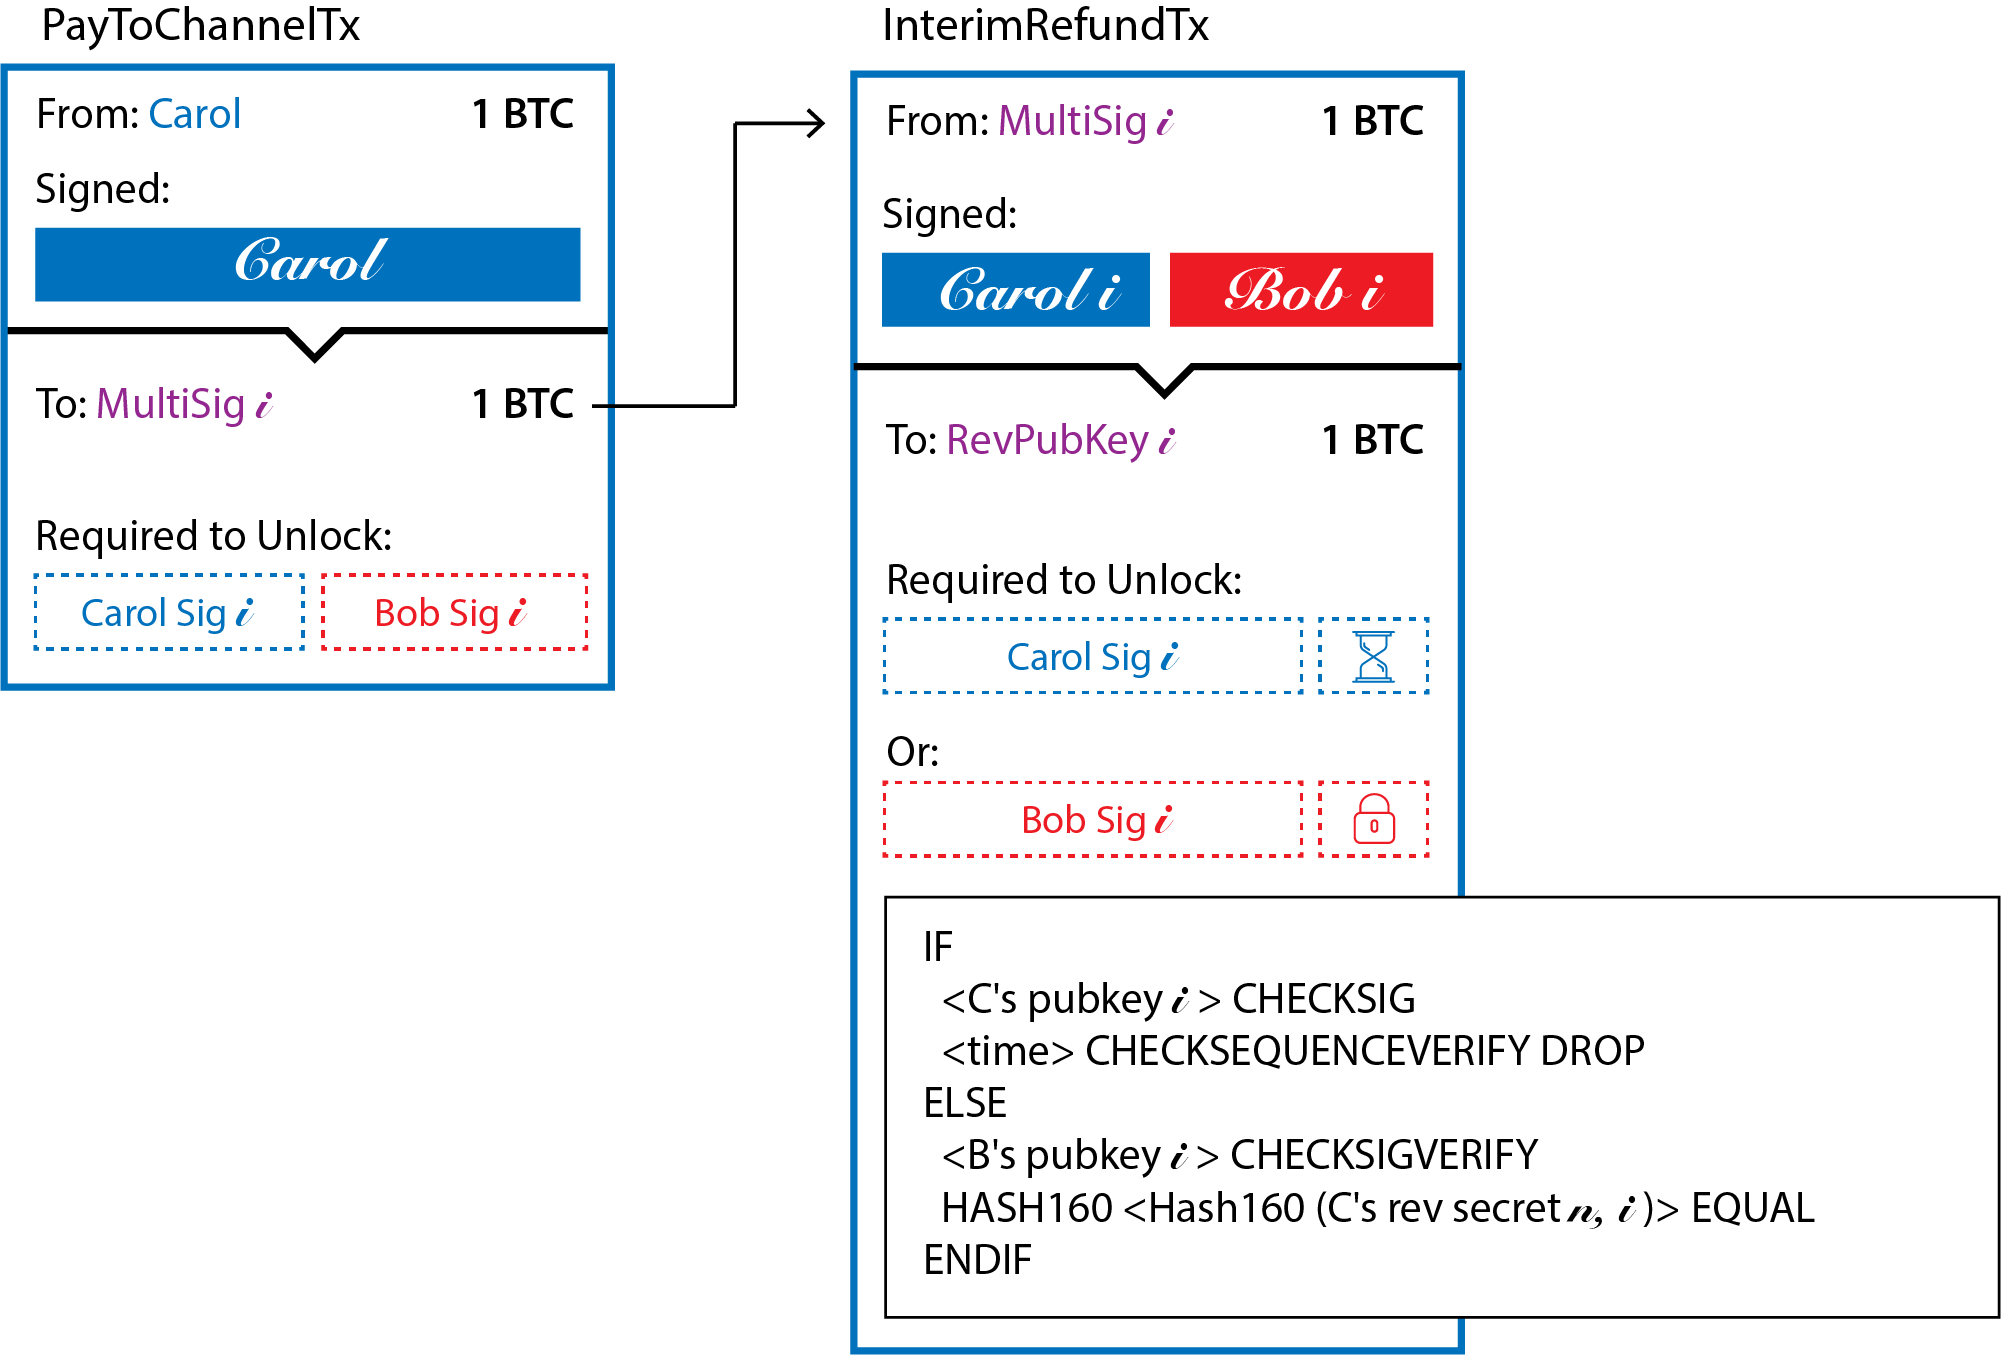
\includegraphics[width=0.65\textwidth]{PayToChannel}
  \caption{Pay to channel transaction by Carol with the interim refund
transaction. The interim refund transaction acts like a standard refund
transaction but aims to be merged in the next round of transactions. The interim
refund transaction has the same spending requirements as a standard refund
transaction, if no transaction is made Carol can spend the interim refund,
otherwise Bob can revoke the interim refund.}
\end{figure}

This transaction automatically settles the channel with the amount owned by Bob
at $\texttt{Channel}_{i,n}$ and changes the remaining amount available for Carol
for the state $\texttt{Channel}_{i+1,n}$, thus, remaining funds are moved to the
next channel address.

\subsubsection{Closed Channel Transaction} The close channel transaction,
hereinafter also mentioned as $\texttt{ClosedChannelTx}_{i}$, is also a
cooperative transaction, that allows Carol or Bob to close the channel in the
most effective way (less fee and quicker). This transaction has two outputs, one
for Bob with the amount owned by Bob to his address and a second one for Carol
with the remaining amount of money in the channel. When a
$\texttt{ClosedChannelTx}_{i}$ is created, no more transactions can be created
or accepted on the channel.

\subsubsection{Pay To Channel Transaction} The pay to channel transaction,
hereinafter $\texttt{PayToChannelTx}_{i}$, allows Carol or Bob to send money
directly to the current channel address. This transaction is useful for Carol if
there is not enough money on the channel and she wants to send more money to Bob
without opening another payment channel. It is also useful for Bob in the case
he wants to send her money and to allow her to reuse it in the channel. He could
send money directly to Carol's address, but the payment might be related to a
channel event or action, e.g fidelity points.

\begin{figure} \centering 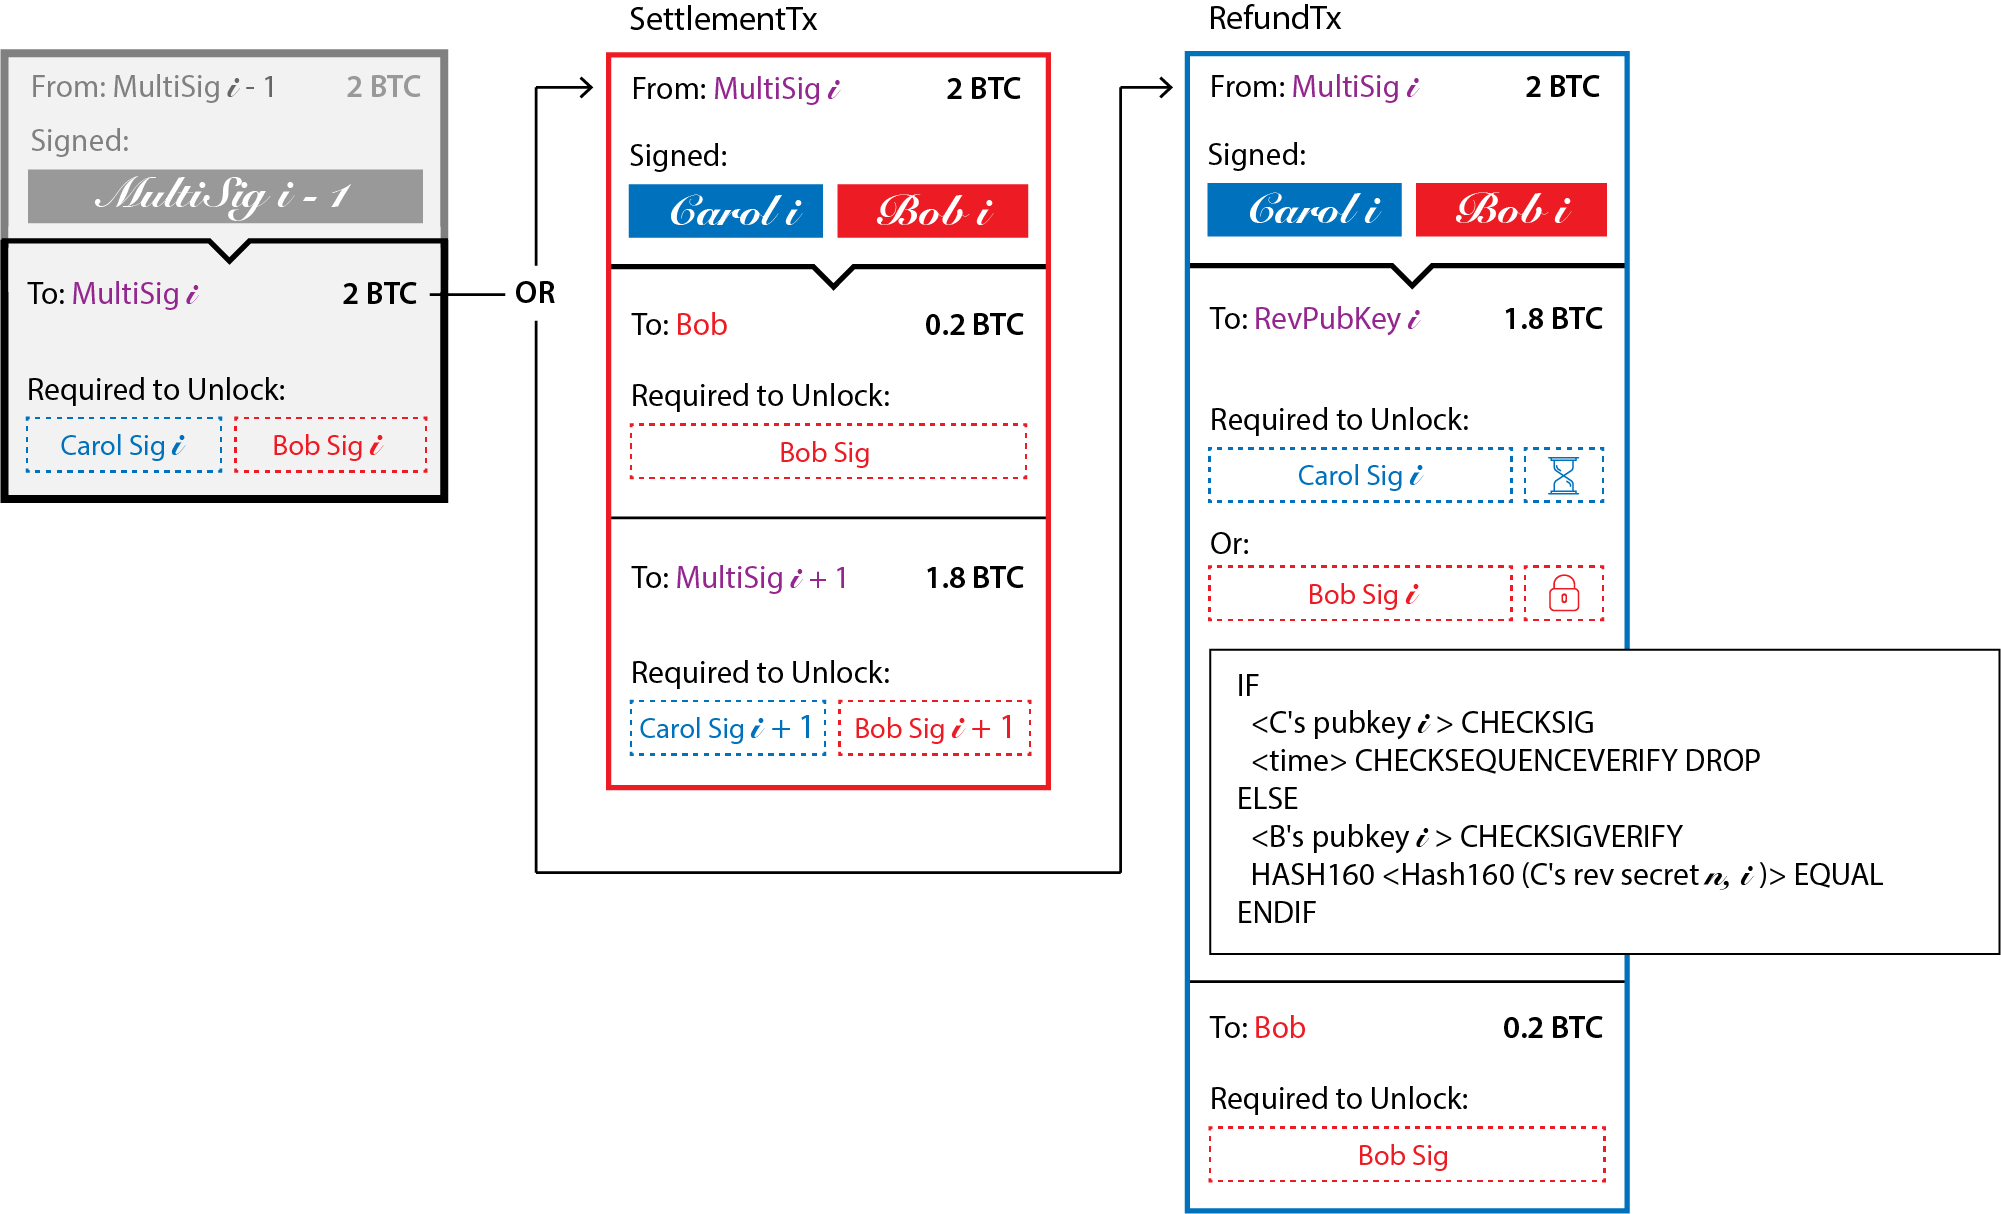
\includegraphics[width=1\textwidth]{StandardState}
  \caption{Simplified view of possibilities for a standard state
$\texttt{Channel}_{i,n}$ without second layer dependency transactions like spend
and revoke. The content of a multisig can be settled by Bob or can be refunded
to Carol.}
\end{figure}

Before broadcasting the pay to channel transaction or before accepting that
payment as part of the usable funds for Carol, an interim refund transaction
needs to be created. This interim refund transaction is a safety guarantee for
Carol until the merge occurs.

For a state $\texttt{Channel}_{i,n}$ without any pay to channel transaction, the
multisig address usually has one unspent output. This unspent output is used as
an input for each transaction and these transactions split it to track the
balances of each party. After a pay to channel transaction, the multisig address
has more than one unspent output. When Carol sends money to Bob they have to
check if a pay to channel transaction occured. In this case they need to merge
the interim refund and use all the unspent outputs. It is worth noting that the
more pay to channel transactions occur the more (fee) cost incurred.

\begin{figure} \centering
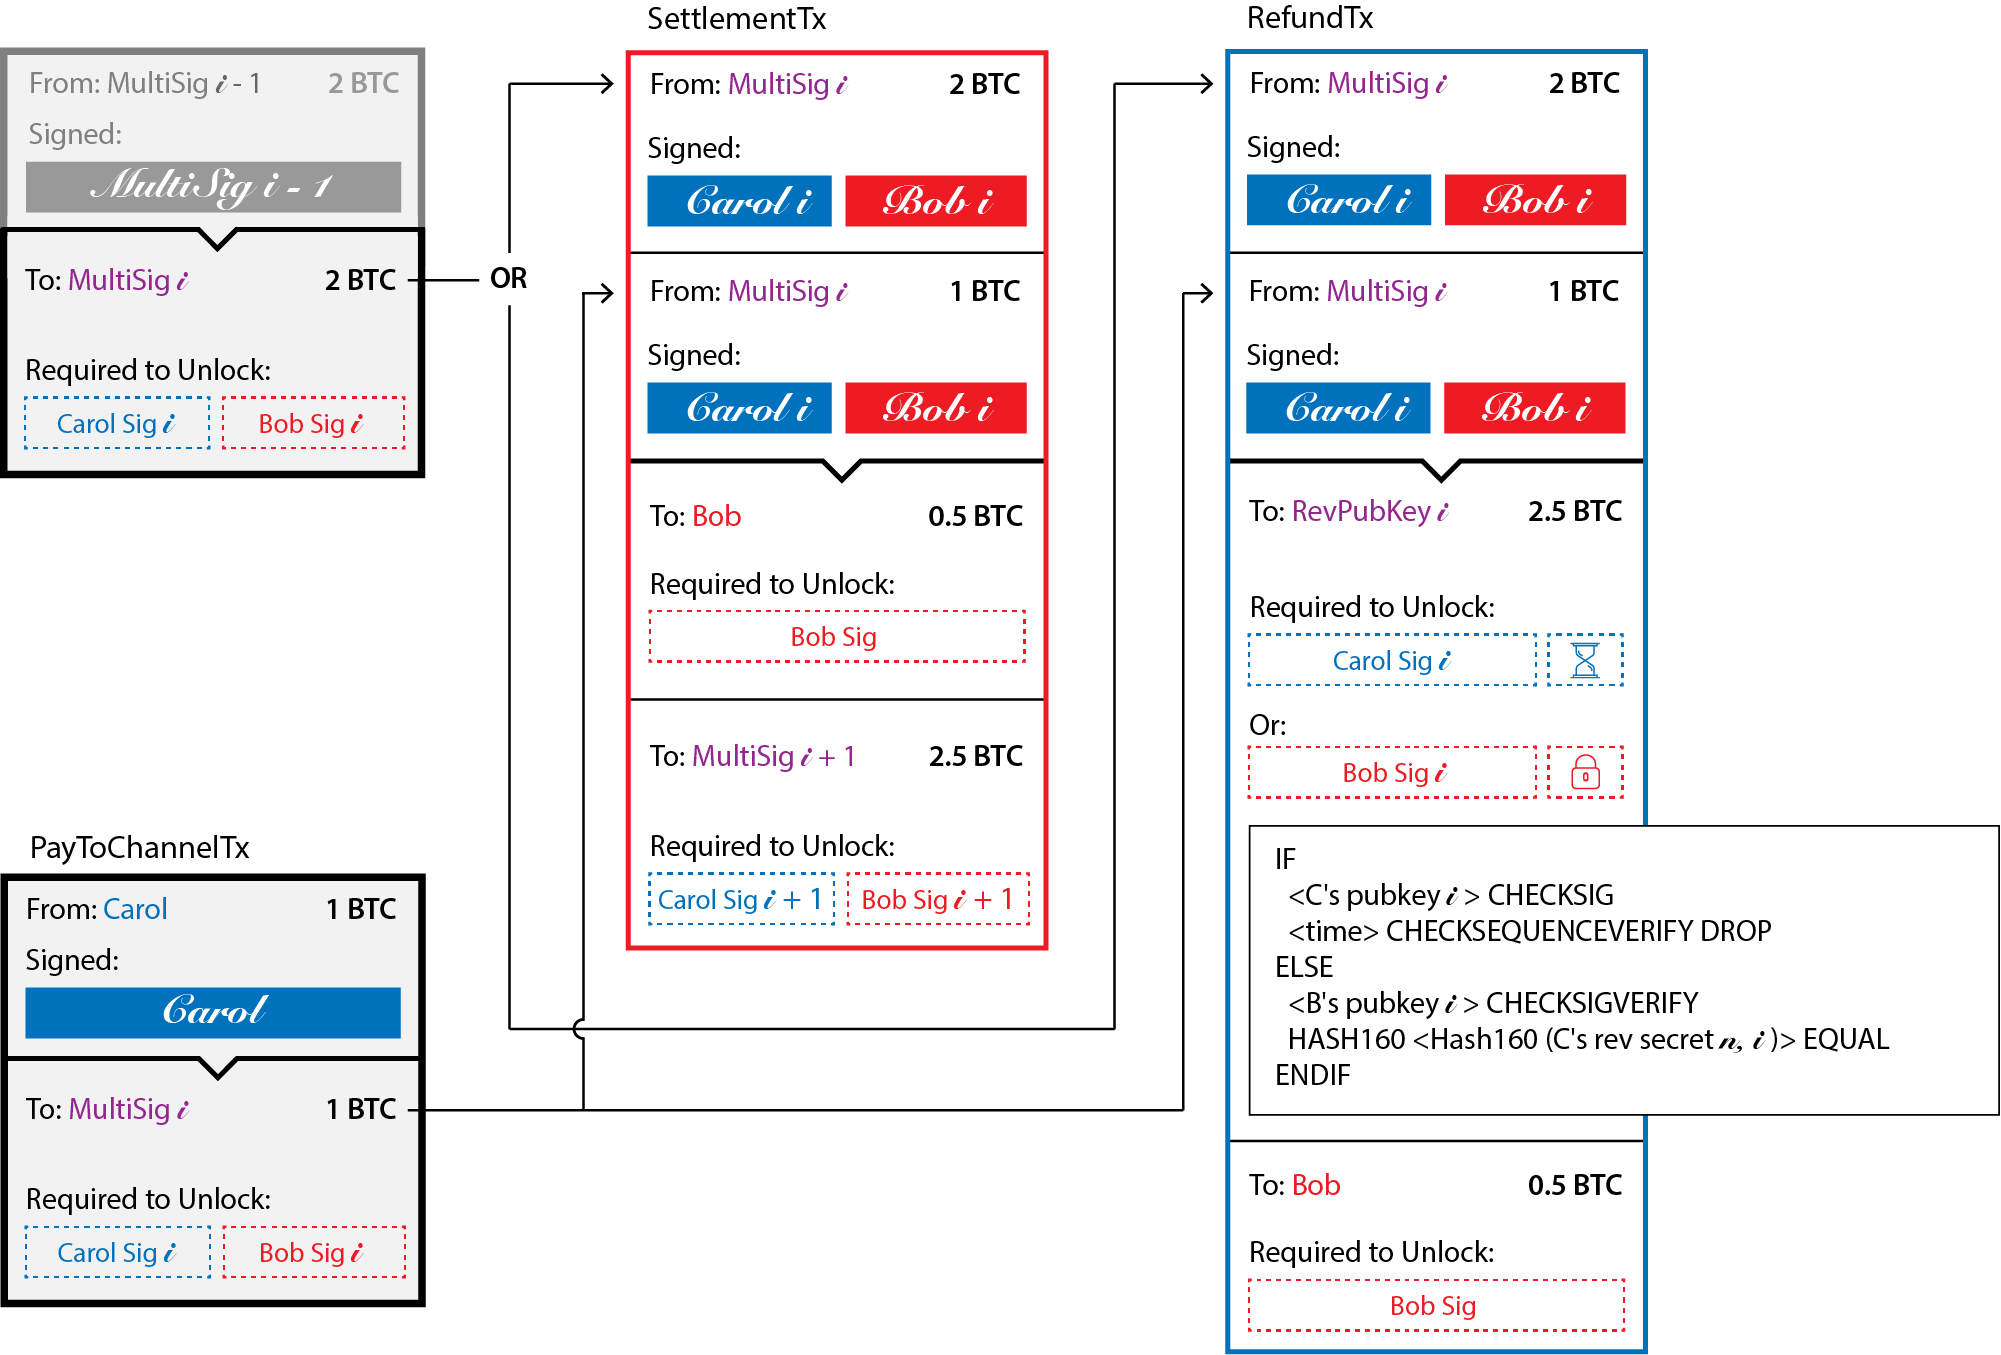
\includegraphics[width=1\textwidth]{MergedPayToChannel}
  \caption{Result of a merged pay to channel transaction after Carol sends more
Bitcoin to Bob. The $\texttt{Multisig}_{i}$ contains two \texttt{UTXOs}, (i)
from the funding transaction or the last move from $\texttt{Multisig}_{i-1}$,
and (ii) from the pay to channel transaction adding 1 BTC into the channel. Both
the settlement transaction and refund transaction contain the two \texttt{UTXOs}
as inputs to sign and spend the totality with the adjusted balances.}
\end{figure}

\subsubsection{Interim Refund Transaction} The interim refund transaction,
hereinafter $\texttt{InterimRefundTx}_{i,n}$, is a temporary transaction used by
Carol to get her money out of the channel. This transaction is created to
protect Carol from Bob invalidating the current refund transaction.

If an unconfirmed Bob to Carol transaction exists and is needed because the
regular multisig address is empty, then the refund must be merged into a new
$\texttt{Channel}_{i,n+1}$ state. Bob can trust this unconfirmed output because
it comes from himself.

\begin{definition}[Channel merge] A channel merge occurs each time an interim
refund transaction is merged into the regular refund transaction and the regular
settlement transaction.
\end{definition}

\begin{definition}[Channel reduce] A channel reduce occurs each time a
non-closing channel transaction is broadcast and included in the blockchain. The
channel is then in reduced mode when one and only one \texttt{UTXO} is available
in the current multisig address.
\end{definition}

\section{Partially Non-Interactive and Instantaneous Channel}

In the following, we describe the protocol layer. The protocol layer enforces
the trustlessness of the channel for every player at each step. A player is safe
as long as he follows this protocol.

\subsection{Channel Setup} Before opening the channel Carol and Bob need to
exchange keys for the channel account $a$ and negotiate the relative timelock
value.

\begin{enumerate}
\item Carol:
  \begin{enumerate}
  \item sends a request to open a channel with:
    \begin{enumerate}
    \item the account $a$
    \item Carol's $\texttt{xPub}_{a}$
    \item the relative timelock parameter
    \end{enumerate}
  \end{enumerate}
\item Bob:
  \begin{enumerate}
  \item if Bob agrees with the request and timelock is whithin acceptable range,
respond with:
    \begin{enumerate}
    \item Bob's $\texttt{xPub}_{a}$
    \end{enumerate}
  \end{enumerate}
\end{enumerate}

\subsection{Channel Opening} To open the channel, Carol and Bob must cooperate
to generate and fund a multi-signature address, hereinafter also referred to as
$\texttt{Multisig}_{i}$ address. This multi-signature address acts as the
channel address and stores the totality of the channel's funds. This address
generally holds only one \texttt{UTXO}, but with pay to channel transactions,
this could be different.

\begin{enumerate}
\item Bob:
  \begin{enumerate}
  \item generates $\texttt{Multisig}_{i}$ with Bob's $\Pi_{i}$ and Carol's
$\pi_{i}$ and sends it
  \end{enumerate}
\item Carol:
  \begin{enumerate}
  \item creates $\texttt{FundingTx}_{<>}^{i}$ that funds the
$\texttt{Multisig}_{i}$ address
  \item generates $\Phi_{i,n}$
  \item creates $\texttt{RefundTx}_{<>}^{i,n}$ with $\texttt{Multisig}_{i}$ and
$\Phi_{i,n}$ sending the full amount back to herself via the
$\texttt{RevPubKey}_{i,n}$ contract
  \item initiates the channel by sending:
    \begin{enumerate}
    \item $\texttt{hash}(\Phi_{i,n})$
    \item $\texttt{RefundTx}_{<>}^{i,n}$
    \end{enumerate}
  \end{enumerate}
\item Bob:
  \begin{enumerate}
  \item receives $\texttt{RefundTx}_{<>}^{i,n}$, signs it and returns
$\texttt{RefundTx}_{<bob>}^{i,n}$
  \end{enumerate}
\item Carol:
  \begin{enumerate}
  \item broadcasts $\texttt{FundingTx}_{<carol>}^{i}$
  \end{enumerate}
\item Bob:
  \begin{enumerate}
  \item waits for transaction's confirmations
  \item consider the channel as open
  \end{enumerate}
\end{enumerate}

If Bob stops responding after step 2, Carol has created transactions which she
is unable to use. If Carol stops responding after step 3, Bob has signed a
transaction which will probably never be used. After a while, Bob must consider
the channel opening as failed. If Bob stops responding after step 4, Carol can
broadcast her refund transaction and she is safe. If Carol stops responding
after opening the channel Bob does not lose anything.

% \begin{figure}
%   \centering
%   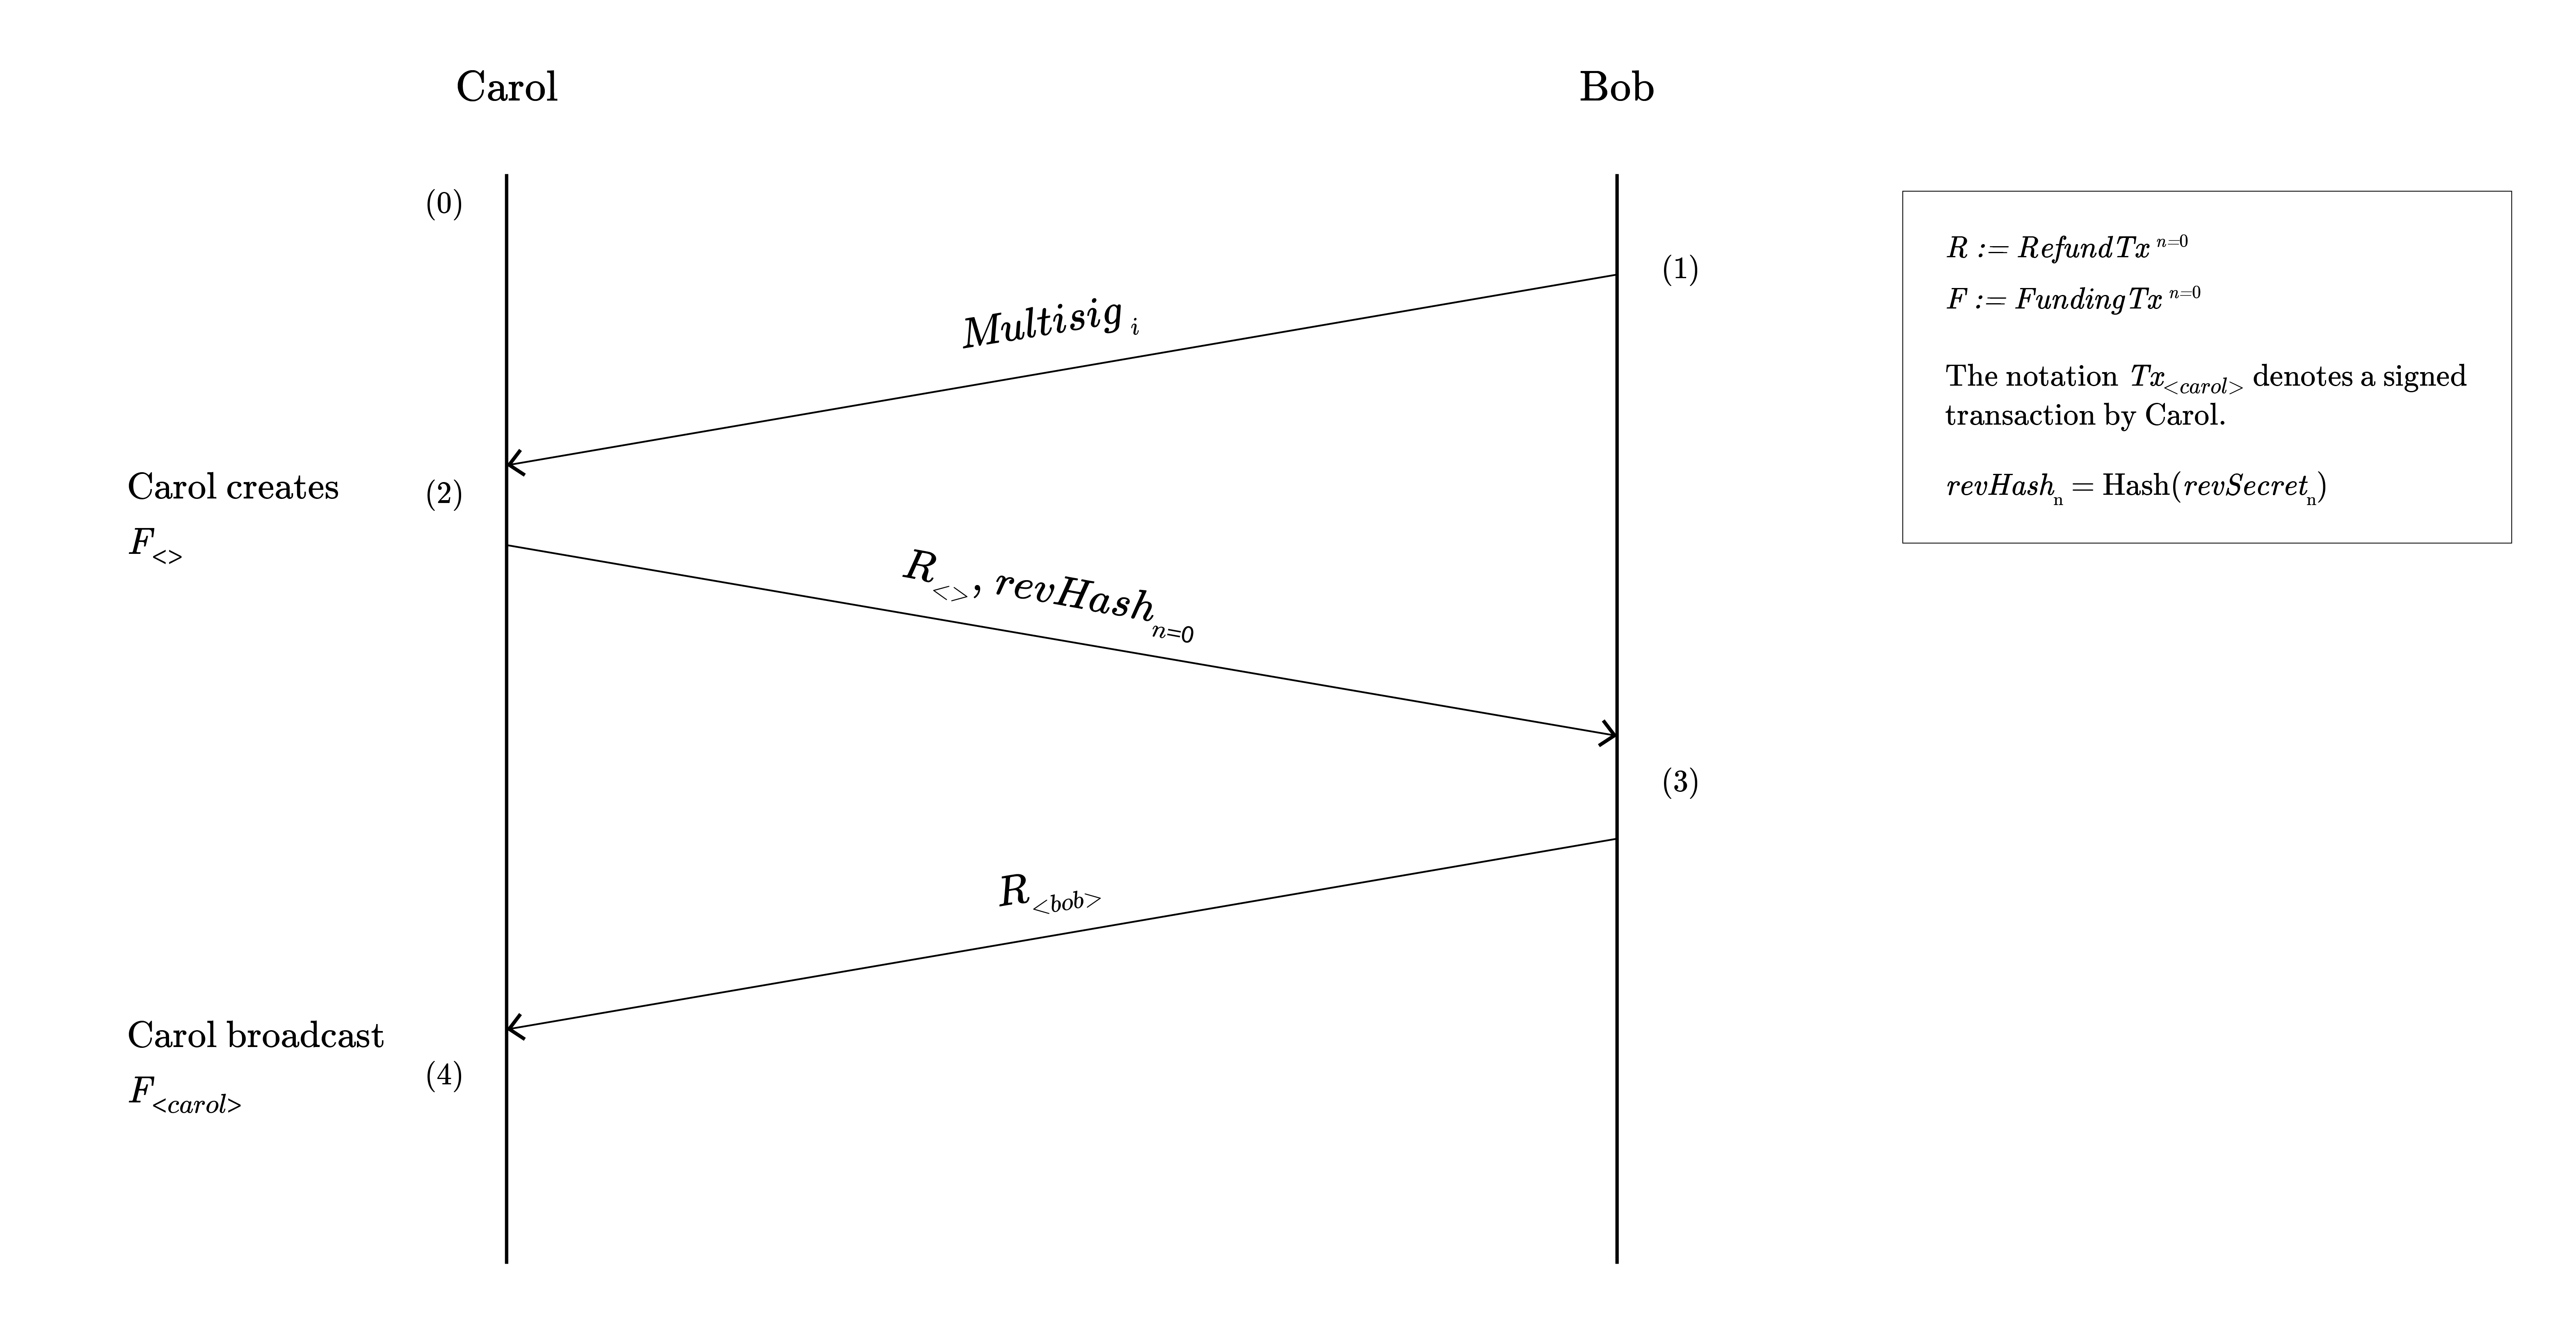
\includegraphics[width=1\textwidth]{payment-channel-opening-01}
%   \caption{Channel opening protocol messages exchange}
% \end{figure}

\subsection{Transact}
\subsubsection{Carol to Bob} The Carol to Bob protocol allows Carol to send an
arbitrary amount of money through the channel, as far as the amount is smaller
than or equal to the funds locked on the $\texttt{Multisig}_i$ address. Carol
desires to authorize a payment of $M$ satoshis to Bob at
$\texttt{Channel}_{i,n}$ state.

\begin{enumerate}
\item Carol:
  \begin{enumerate}
  \item derives $\Phi_{i,n+1}$ and $\Phi_{i+1,n+1}$
  \item generates the $\texttt{RefundTx}_{<>}^{i,n+1}$ with two outputs:
    \begin{enumerate}
    \item Refund Output: Carol's new balance to $\texttt{RevPubKey}_{i,n+1}$
contract
    \item Settlement Output: Bob's new balance to settlement address
    \end{enumerate}
  \item sends a message to Bob containing:
    \begin{enumerate}
    \item $\texttt{RefundTx}_{<>}^{i,n+1}$
    \item $\texttt{hash}(\Phi_{i,n+1})$ and $\texttt{hash}(\Phi_{i+1,n+1})$
    \item the amount of $M$ satoshis being paid
    \end{enumerate}
  \end{enumerate}
\item Bob:
  \begin{enumerate}
  \item generates the $\texttt{SettlementTx}_{<>}^{i}$ with two outputs:
    \begin{enumerate}
    \item Settlement Output: Bob's new balance
    \item Change Output: Carol's new balance to $\texttt{Multisig}_{i+1}$ with
Bob's $\Pi_{i+1}$ and Carol's $\pi_{i+1}$
    \end{enumerate}
  \item generates the $\texttt{PostSettlementRefundTx}_{<bob>}^{i+1,n+1}$ with:
    \begin{enumerate}
    \item Refund Output: sends Carol's funds to the associated
$\texttt{RevPubKey}_{i+1,n+1}$ contract with the secret $=
\texttt{hash}(\Phi_{i+1,n+1})$
    \end{enumerate}
  \item sends:
    \begin{enumerate}
    \item $\texttt{RefundTx}_{<bob>}^{i,n+1}$
    \item $\texttt{SettlementTx}_{<>}^{i}$
    \item $\texttt{PostSettlementRefundTx}_{<bob>}^{i+1,n+1}$
    \end{enumerate}
  \end{enumerate}
\item Carol:
  \begin{enumerate}
  \item sends:
    \begin{enumerate}
    \item $\texttt{SettlementTx}_{<carol>}^{i}$
    \item the shared secret $\Phi_{i,n}$
    \end{enumerate}
  \end{enumerate}
\item Bob:
  \begin{enumerate}
  \item upates state channel to $\texttt{Channel}_{i,n} \Rightarrow
\texttt{Channel}_{i,n+1}$ and the payment can now be considered as final
  \end{enumerate}
\end{enumerate}

If Bob stops responding after step 2, Carol can broadcast the refund transaction
but she has no incentives to do that because she will lose part of her balance
compared to broadcasting the previous state refund transaction.

Because she has not yet shared the secret $\Phi_{i,n}$, Bob cannot yet revoke
the current $\texttt{Channel}_{i,n}$ state. If Carol does not respond at step 3,
Bob can settle the current $\texttt{Channel}_{i,n}$ state, but cannot settle the
$\texttt{Channel}_{i,n+1}$ state in negotiation, Carol is safe. After step 3,
Carol can refund herself and Bob can revoke the old $\texttt{Channel}_{i,n}$
state and settle the new $\texttt{Channel}_{i,n+1}$ state, the transaction is
complete.

\subsubsection{Channel Top-up} The channel top-up protocol allows Bob or Carol
to send an output directly to the current channel multisig address and allows
Carol to include this output as part of usable funds immediately if it is from
Bob. If the funds come from Carol, they can be immediatley used for a withdraw
transaction only.

To protect Carol, the refund for this additional amount is separated from the
existing refund output to prevent Bob from invalidating Carol's refund
transaction by sending an output which becomes invalid or not accepted by the
network (lower fee, double spend, invalid script, etc.)

In subsequent transactions, once this output has been confirmed, the refund
should be merged into a single refund output as before, to be more efficient
with refund transaction size.

\begin{enumerate}
\item Initiator:
  \begin{enumerate}
  \item create the $\texttt{PayToChannelTx}_{<initiator>}^{i}$ that funds the
$\texttt{Multisig}_{i}$ address
  \item create $\texttt{InterimRefundTx}_{<>}^{i,n}$ with
$\texttt{Multisig}_{i}$ and $\texttt{hash}(\Phi_{i,n})$ sending the full amount
back to Carol via the $\texttt{RevPubKey}_{i,n}$ contract
  \item sends:
    \begin{enumerate}
    \item $\texttt{InterimRefundTx}_{<initiator>}^{i,n}$
    \end{enumerate}
  \end{enumerate}
\item Receiver:
  \begin{enumerate}
  \item validate $\texttt{InterimRefundTx}_{<initiator>}^{i,n}$
  \item sends if the payment is accepted or not
  \end{enumerate}
\item Initiator:
  \begin{enumerate}
  \item if the payment is accepted broadcast
$\texttt{PayToChannelTx}_{<initiator>}^{i}$
  \end{enumerate}
\item Receiver:
  \begin{enumerate}
  \item wait for $\texttt{PayToChannelTx}_{<initiator>}^{i}$ transaction's
confirmations
  \end{enumerate}
\end{enumerate}

If the receiver does not validate the payment, the initiator has no incentives
to broadcast the transaction. If it is accepted, then the initiator can safely
send money into the channel because of the interim refund transaction. Without
negotiating a new state, Bob cannot revoke
$\texttt{InterimRefundTx}_{<initiator>}^{i,n}$ and Carol can spend the refund.
When a new $\texttt{Channel}_{i,n+1}$ state is negotiated, Bob can revoke the
$\texttt{InterimRefundTx}_{<initiator>}^{i,n}$ if Carol tries to broadcast it.
At $\texttt{Channel}_{i,n+1}$, the refund transaction and the settlement
transaction contain the merged refund transaction.

It is worth noting that the initiator does need to know the secret to create the
pay to channel transaction and the interim refund transaction. An external
player can ask the needed information to top-up the channel knowing only public
information.

\subsubsection{Withdrawing} The withdraw protocol allows Bob to authorize a
withdrawal of $M$ satoshis at Carol's request and with her cooperation for
$\texttt{Channel}_{i,n}$ state. Bob needs to validate the withdrawal amount and
can set up a set of rules internally to manage the channel economics. It is
worth noting that when the withdraw takes place Bob funds get automatically
settled without him paying fees.

\begin{enumerate}
\item Carol:
  \begin{enumerate}
  \item derives $\Phi_{i+1,n}$
  \item generates the $\texttt{Multisig}_{i+1}$ address with Bob's $\pi_{i+1}$
and Carol's $\Pi_{i+1}$
  \item generates the $\texttt{WithdrawTx}_{<>}^{i}$ with:
    \begin{enumerate}
    \item Settlement Output: sends Bob's funds to the settlement address
    \item Withdraw Output: withdrawal amount $M$ to specified address
    \item Change Output: new balance into $\texttt{Multisig}_{i+1}$
    \end{enumerate}
  \item generates the $\texttt{RefundTx}_{<>}^{i+1,n}$ from address
$\texttt{Multisig}_{i+1}$ with:
    \begin{enumerate}
    \item Refund Output: Carol's new balance into $\texttt{RevPubKey}_{i+1,n}$
contract with the secret $= \texttt{hash}(\Phi_{i+1,n})$
    \end{enumerate}
  \item sends:
    \begin{enumerate}
    \item $\texttt{RefundTx}_{<>}^{i+1,n}$
    \item $\texttt{WithdrawTx}_{<>}^{i}$
    \item $\texttt{hash}(\Phi_{i+1,n})$
    \end{enumerate}
  \end{enumerate}
\item Bob:
  \begin{enumerate}
  \item verifies, signs and returns:
    \begin{enumerate}
    \item $\texttt{RefundTx}_{<bob>}^{i+1,n}$
    \item $\texttt{WithdrawTx}_{<bob>}^{i}$
    \end{enumerate}
  \end{enumerate}
\item Carol:
  \begin{enumerate}
  \item shares:
    \begin{enumerate}
    \item $\Phi_{i,n}$ to invalidate the current state
    \item $\texttt{WithdrawTx}_{<bob,carol>}^{i}$
    \end{enumerate}
  \end{enumerate}
\item Bob:
  \begin{enumerate}
  \item broadcast $\texttt{WithdrawTx}_{<bob,carol>}^{i}$
  \item upates state channel to $\texttt{Channel}_{i,n} \Rightarrow
\texttt{Channel}_{i+1,n}$ and validate exchange
  \end{enumerate}
\end{enumerate}

If Bob does not respond during step 2, Carol has not disclosed any important
information. If Bob stops responding after step 2, Carol can withdraw the amount
and safely refund her funds if no transaction is negotiated. If Carol does not
respond after step 2, Bob must wait a while and if the withdraw transaction is
not broadcasted, he must broadcast the settlement transaction to force the
transition to the next $\texttt{Channel}_{i+1,n}$ state.

\subsubsection{Settlement} The settlement protocol allows Bob to broadcast at
$\texttt{Channel}_{i,n}$ state the $\texttt{SettlementTx}_{i,n}$ to get the
settlement output and move the remaining funds into the next
$\texttt{Multisig}_{i+1}$ address. In this case the channel stays open and Carol
can create new transactions or close the channel.

If the $\texttt{SettlementTx}_{i,n}$ is broadcast and Carol wants to close the
channel, she can broadcast the $\texttt{PostSettlementRefundTx}_{i,n}$ and wait
the timelock to get her money back. Carol has to query the network to know if
the $\texttt{SettlementTx}_{i,n}$ has been broadcasted, she can only query the
blockchain before each new transaction to be sure that the settlement
transaction has not been broadcasted yet.

\subsection{Channel Closing}
\subsubsection{Cooperative} Closing the channel cooperatively allows Carol---or
Bob if Carol is online---to ask if Bob agrees to close the channel efficiently,
withdrawing the full remaining balance, at $\texttt{Channel}_{i,n}$ state. The
following steps 3 and 4 can be merged and executed by the same player depending
on the implementation.

\begin{enumerate}
\item Carol:
  \begin{enumerate}
  \item generates the $\texttt{ClosedChannelTx}_{<carol>}^{n+1}$ with:
    \begin{enumerate}
    \item Settlement Output: sends Bob's funds to Bob address
    \item Change Output: sends Carol's funds to Carol address
    \end{enumerate}
  \item sends $\texttt{ClosedChannelTx}_{<carol>}^{n+1}$
  \end{enumerate}
\item Bob:
  \begin{enumerate}
  \item verifies and signs $\texttt{ClosedChannelTx}_{<carol>}^{n+1}$
  \item sends $\texttt{ClosedChannelTx}_{<carol,bob>}^{n+1}$
  \end{enumerate}
\item Carol:
  \begin{enumerate}
  \item broadcasts $\texttt{ClosedChannelTx}_{<carol,bob>}^{n+1}$
  \end{enumerate}
\end{enumerate}

\subsubsection{Contentious} The contentious channel closing protocol allows
Carol to close the channel alone, i.e., without Bob's cooperation or response,
at $\texttt{Channel}_{i,n}$ state. Carol can broadcast her fully signed refund
transaction sending her funds to $\texttt{RevPubKey}_{i,n}$ address. Carol would
then need to spend from the revocation public key contract after the timelock
delay with the spend refund transaction.

\textit{It is worth noting that only Carol can close the channel, but Bob can
get his money by broacasting his settlement transaction at any time.}

For state $\texttt{Channel}_{i,n}$, Bob can broadcast his fully signed
settlement transaction to get his money back, but Bob cannot close the
channel. In that case Carol, if she want, can broadcast her fully signed post
settlement transaction at any time to close the channel. Carol would then need
to spend from $\texttt{RevPubKey}_{i,n}$ after the timelock delay.

\section{Evidence of Trustlessness} In the following, axioms, possible
edge-cases, and discovered attacks, with an evidence of trustlessness for the
channel protocol, are exposed. \textit{Liveness} in the blockchain is a
prerequisite to guarantee the security model. That is, broadcasted transactions
are assumed to get included in the blockchain within a predictable time delay.

\subsection{Axioms}

\subsubsection{Refund Transaction} For $\texttt{Channel}_{i,n}$ state, if Carol
broadcasts the current refund transaction, Bob cannot revoke it without knowing
$\Phi_{i,n}$. After the timelock, Carol can generate and broadcast a spend
refund transaction.
\[ \forall (i,n) \exists \Phi_{i,n} | \text{Bob knows } \Phi_{i,n-1}
\text{ and } \texttt{hash} ( \Phi_{i,n} )
\]

The same rule is applied to interim refund transactions, if Carol broadcasts the
current interim refund transaction, Bob cannot revoke it without knowing
$\Phi_{i,n}$, and Carol can spend the interim refund after the timelock.

\subsubsection{Old Refund Transaction} For $\texttt{Channel}_{i,n}$ state, if
Carol broadcasts an old refund transaction, e.g. $n-1$, then Bob has the time
during the timelock to generate and broadcast the revoke transaction for the
state $\texttt{Channel}_{i,n-1}$ with $\Phi_{i,n-1}$ secret.
\[ \forall x \in \{1,\dots,n-1\} \exists \texttt{RevokeTx}_{<bob>}^{i,x}
\]

The same rule is applied to old interim refund transactions, if Carol broadcasts
an old interim refund transaction, e.g. $n-1$, Bob can revoke it with
$\Phi_{i,n-1}$ secret.

\subsubsection{Settlement Transaction} For $\texttt{Channel}_{i,n}$ state, if
Bob broadcasts his transaction $\texttt{SettlementTx}_{i,n}$, Carol has the
choice to close the channel or transact on top of the new
$\texttt{Multisig}_{i+1}$ address.
\[ \forall \texttt{Channel}_{i,n} \exists \Phi_{i,n} \text{ and } \exists
\Phi_{i+1,n}
\]
\[ \text{Bob knows } \Phi_{i+1,n} \iff \exists\texttt{Channel}_{i+1,n+1}
\]

\subsubsection{Contentious Channel Closing} By contentious it is meant that all
players are not communicating anymore and/or do not agree on a valid state.
Let's define the way for Carol to close the $\texttt{Channel}_{i,n}$ state.
\[ \forall \texttt{Channel}_{i,n} \exists \texttt{RefundTx}_{<carol,bob>}^{i,n}
\text{only owned by Carol}
\] and
\[ \forall \texttt{RefundTx}_{<carol,bob>}^{i,n} \exists
\texttt{SpendRefundTx}_{<carol>}^{i,n} \text{only owned by Carol}
\] so
\[ \forall \texttt{Channel}_{i,n} \exists
\texttt{SpendRefundTx}_{<carol>}^{i,n} \text{only owned by Carol}
\]

\subsection{Edge Cases}

\subsubsection{Someone does not broadcast Cooperative Transaction} If one player
does not share a fully signed cooperative transaction and the secret
$\Phi_{i,n}$ attached to the current $\texttt{Channel}_{i,n}$ state, then the
other player eventually needs to force the transition into the new
$\texttt{Channel}_{i+1,n}$ state with his own fully signed transaction, i.e
$\texttt{RefundTx}_{i,n}$ or $\texttt{SettlementTx}_{i,n}$ transaction.

\subsection{Attacks} In this section, discovered attack vectors and fixes are
discussed. Attacks exposed are no longer valid in the current scheme, but a deep
analysis has been carried out to generalize the protocol construction and
improve the scheme.

\subsubsection{Old Settlement Attack With Weak Secret}
\label{sssec:oldSettlementAttack} It is possible for Bob to lock the funds in
the multisig or steal the money if the secret construction is too weak. For a
$N$ dimensions channel the secret is considered weak if
\[ |\Phi| < N
\]

Let's assume that the revocation secret $\Phi$ only depends on $n$ and not on
$i$ for $\texttt{Channel}_{i,n}$. Hence, the secret can be expressed as
\[ |\texttt{Channel}_{i,n}| = N = 2 : |\Phi_n| = 1 \implies |\Phi_n| < N
\]

Then, for $\texttt{Channel}_{i,n}$, if Bob broadcasts an old settlement
transaction, e.g. $n-1$, then Carol cannot use her post settlement refund
transaction because she previously shared the secret $\Phi_{n-1}$. So the
remaining funds are blocked in the $\texttt{Multisig}_{i+1}$ address. To be able
to get her funds back, Carol would have to transact with Bob. If Bob does not
cooperate, Carol has no way to recover her funds. If she tries to refund the
$\texttt{Multisig}_{i+1}$, then Bob can revoke it with $\Phi_{n-1}$ secret.

If dimension of used secret is equal to the channel dimension, i.e.
$|\Phi_{i,n}| = |\texttt{Channel}_{i,n}|$, then the previous shared secret is
$\Phi_{i,n-1}$ and the secret for refunding the $\texttt{Multisig}_{i+1}$
address at $\texttt{Channel}_{i,n-1}$ state is $\Phi_{i+1,n-1}$ and therefore
\[ \Phi_{i,n-1} \neq \Phi_{i+1,n-1}
\]

Game theory is not sufficient to ensure the security of the channel; if, when a
player acts dishonestly, there exists an incentive to gain, even
probabilistically, over the other player. In this case, the provider loses funds
by broadcasting the $\texttt{Channel}_{i,n-1}$ state but can gain all funds if
the client does not act correctly and does unlock his funds.

\subsubsection{Secret Size Attack} A recent advisory notes a vulnerability in
the common construction of cross-chain smart contracts (contracts between
distinct cryptocurrencies) through hash locking \cite{SecretSizeAttack}. It
focus on the primary use case in atomic swap contracts, which allow two
cryptocurrencies to changes hands simultaneously and safely. The vulnerability
can be generalized to a secret $s$ and its hash $h = \texttt{hash}(s)$ generated
by a player $p_1$ but required by another player $p_2$. When player $p_1$ send
the hash $h$ to player $p_2$, $p_2$ do not has the possibility to assert the
validity of $h = \texttt{hash}(h)$.

Our scheme is not affected by this attack. In the protocol Carol generates the
revocation secret, send the corresponding hash to Bob, and Bob assumes that a
valid secret exists and is known by Carol. Bob use the received hash to create
and validate  the first transaction and accept the payment. When the second
transaction occurs Bob receive the new hash and the previous secret. At this
moment he can validate  if a revocation secret exists and is valid, otherwise
Bob refuses the new payment and Carol has no choice but closing the channel
cooperatively or not.

\section{Further Improvements} Improvements can be done in two ways: (i)
extending channel capabilities or (ii) optimizing the channel costs by reducing
the transaction size or occurences.

\subsection{Threshold Signatures} The ability to settle and withdraw the channel
without closing has a downside. Each time a transaction is broadcast on chain, a
fee is charged. Optimizing the channel transaction size or the number of
transactions needed is an area of further research.

The main cost of a transaction comes from its inputs and their types. A channel
transaction spends one or more \texttt{UTXOs} from the $\texttt{Multisig}_{i}$
address. These \texttt{UTXOs} are \texttt{P2SH} of a Bitcoin 2-out-of-2
multi-signature script that requires, obviously, two signatures. Knowing that a
signature size is at least 64 bytes and an average transaction size (one simple
input and one or two outputs) is a bit more than 200 bytes, it is easy to see
that replacing the \texttt{P2SH} with a 2-out-of-2 multisig \texttt{UTXOs} by
\texttt{P2PKH} \texttt{UTXOs} is more efficient in any case.

Three transactions are compared with SegWit\footnote{ The transaction size
is calculated with nested-SegWit and not with native mode} and without.
Optimization is expressed in percentage of size or virtual-size economized. The
Script Hash (SH) consumes a multi-signature script, and the Public Key Hash
(PKH) consumes a standard public key. Note that size can vary by a few bytes
with SegWit.

The average fee per virtual byte in the last three months was around 292
Satoshis. This optimization allows savings of up to 32,412 Satoshis for the
first refund transaction without SegWit, and 12,264 Satoshis for a refund
or a settlement transaction with SegWit. At the current price, these
savings represent between USD \$1.31 and USD \$3.47\footnote{ Average price of
Bitcoin in the last 3 months, around \$10,700 USD end of 2017}. If the channel is used for
micropayments such as a couple of cents each time, this optimization makes a
difference and lowers the required threshold for feasibility. The first refund
transaction being less expensive also makes the clients commitment easier. The
Table~\ref{fig:summaryTransactionSizeOpti} exhibits transaction utilizing only
one input, and it is worth noting that the number of input has a supralinear
influence to the savings.

\begin{table}[t]
  \begin{tabularx}{\textwidth}{| X | S | S | S | S | S | S |}
  \cline{3-7}
  \multicolumn{2}{l|}{ } & \multicolumn{2}{c|}{Non-SegWit} &
  \multicolumn{3}{c|}{SegWit} \\ \hhline{~~-----}
  \multicolumn{2}{l|}{ } & R-Size & O & \cellcolor[gray]{0.9} R-Size &
  V-Size & O \\ \hhline{--=====}
  \multirow{2}{*}{First Refund}  & SH   & 302  & \multirow{2}{*}{36.75\%} &
  \cellcolor[gray]{0.9} 340 & 174  & \multirow{2}{*}{22.99\%}\\ \hhline{~--~--~}
  & PKH  & 191  & & \cellcolor[gray]{0.9} 216 & 134  & \\ \hhline{-------}
  \multirow{2}{*}{Refund Normal} & SH   & 335  & \multirow{2}{*}{32.54\%} &
  \cellcolor[gray]{0.9} 372 & 207  & \multirow{2}{*}{20.29\%}\\ \hhline{~--~--~}
  & PKH  & 226  & & \cellcolor[gray]{0.9} 246 & 165  & \\ \hhline{-------}
  \multirow{2}{*}{Settlement}    & SH   & 335  & \multirow{2}{*}{32.54\%} &
  \cellcolor[gray]{0.9} 372 & 207  & \multirow{2}{*}{20.29\%}\\ \hhline{~--~--~}
  & PKH  & 226  & & \cellcolor[gray]{0.9} 246 & 165  & \\ \hhline{-------}
  \end{tabularx}

  \medskip
  \caption{Summary of transaction size optimization}
  \label{fig:summaryTransactionSizeOpti}
\end{table}

Requirements need to be defined to be able to substitute the multi-signature
script with a threshold scheme. Analysis of the protocol and the signing process
for a multi-signature script allows one to define these requirements. A
2-out-of-2 multi-signature script can be unlocked with two different public keys
and their signature. The signing order only matters in that it is determined at
the time of creating a multisig address. Some standards such as BIP45
address the need to predefine or communicate the ordering of the keys (and
therefore the signatures) by always ordering the keys lexicographically, and
always ordering the signatures in order of the keys \cite{BIP45}. The protocol
takes advantage of this fact. A transaction is usually held fully signed only by
one player. The threshold scheme must follow these requirements (i) 2 players
need to co-operate to generate a valid signature, (ii) both must be able to
start the signing process, and (iii) only one player must be able to retrieve
the signature at the end of the process. If both need the signature it is always
feasible to share, meaning the current protocol is not better in this case.

To achieve this, an ECDSA threshold signature scheme, with the same requirements
as the 2-out-of-2 multisig, is required. This scheme exists and can be adapted
from the paper \say{Two-Party Generation of DSA Signatures} by MacKenzie and
Reiter \cite{10.1007/3-540-44647-8_8}.

\subsection{Pre-authorized Payments} Pre-authorized payments are required in
other real case scenarios such as provider acting as a payment processor. The
client must be able to set a limit within which the provider can take money.

Further research can be done in this area to figure out the feasibility and the
most effective way to implement this feature in this scheme. Maybe a third
layer, on top of layer two, is necessary and achievable, maybe the channel
dimension can be increased.

\section{Related Work} Simple micropayment channels were introduced by Hearn and
Spilman \cite{Bitcoin_contracts}. The Lightning Network by Poon and Dryja
\cite{lightningNetwork}, also creates a duplex micropayment channel. However it
requires exchanging keying material for each update in the channels, which
results in either massive storage or computational requirements in order to
invalidate previous transactions. Finally, Decker and Wattenhofer introduced a
payment network with duplex micropayment channels
\cite{10.1007/978-3-319-21741-3_1}.

\section{Conclusion} Trustless one-way payment channels for Bitcoin resolve many
problems. Scalability is near infinite and costs of the channel decrease
linearly with the number of transactions in the channel. Delays to consider a
transaction as valid are brought back to network delay and minimal check time.
Clients do not need to be online to keep their funds safe in the channel and can
withdraw arbitrary amounts and refill the channel at any time. The provider does
not need to lock funds to receive money and has no cost to setup a channel with
a client.

\section{Acknowledgement} Loan Ventura, Thomas Roulin and Nicolas Huguenin are
acknowledged for their helpful contribution and comments during the completion
of this work.

%
% ---- Bibliography ----
%
\printbibliography

% % % % ---- Appendix ---- % %
% \newpage % \newgeometry{top=20mm, bottom=20mm, left=20mm, right=20mm}
% \begin{landscape}
% \appendix
% \section{Transaction Dependency Graph} %
% \includegraphics[width=24cm]{payment-channel-08}
% \end{landscape} % \restoregeometry

\end{document}
